
\documentclass[a4paper,fontsize=12pt,headsepline]{scrartcl}



\usepackage{graphicx}
\usepackage[usenames]{color}

\usepackage[english]{babel}  
\usepackage[automark]{scrlayer-scrpage}
\usepackage{setspace}

\usepackage{float}
\usepackage{subcaption}  %%% newer version that can be used instead of subfigure
\usepackage[section]{placeins}

\usepackage{geometry}
\usepackage{url}


\usepackage{texshade} % MSA prints
\usepackage[]{amsmath} % Amsmath - Mathematik Basispaket
\usepackage{amssymb}

%%%%%%%%%% bibliography %%%%%%%%%%%%%%%%%%%%%%%%%%%%%%%
\usepackage[authoryear, sort, square]{natbib}
\bibliographystyle{cell}
%\usepackage[%
%	square,	% for square brackets;
%	comma,	% to use commas as separaters;
%	numbers,	% for numerical citations;
%	sort,		% orders multiple citations into the sequence in which they appear in the list of references;
%	sort&compress,    % as sort but in addition multiple numerical citations
%]{natbib}

%spaces between single entries
%\setlength{\bibsep}{3pt}
%%%%%%%%%%%%%%%%%%%%%%%%%%%%%%%%%%%%%%%%%%%%%%%%%%%%%


%\usepackage{subfig} % Layout wird weiter unten festgelegt !
%\usepackage{subfigure} % Layout wird weiter unten festgelegt !
% Aussehen der Captions fuer subfigures (subfig-Paket)
\usepackage[english,intoc]{nomencl}
%\usepackage{url} % Setzen von URLs. In Verbindung mit hyperref sind diese auch aktive Links.
\usepackage{ae} %erkennt umlaute
% sz
%\usepackage[latin1]{inputenc} 
\usepackage[utf8]{inputenc}

%\usepackage{caption}
\usepackage[font={sf,bf,small},textfont=md,textfont=md]{caption} 

% Aussehen der Captions
\captionsetup{
   margin = 5pt,
   font={sf,bf,small},
   textfont = {md,small},
   format = default, %singlespace% oder 'hang'
   indention = 0em,  % Einruecken der Beschriftung
   %labelsep = colon, %period, space, quad, newline
   %justification = RaggedRight, % justified, centering
   singlelinecheck = true, % false (true=bei einer Zeile immer zentrieren)
   position = bottom %top
}
%%% Bugfix Workaround
\DeclareCaptionOption{parskip}[]{}
\DeclareCaptionOption{parindent}[]{}
%\DeclareCaptionLabelFormat{andtable}{#1~#2 \& \tablename~\thetable}

% Aussehen der Captions fuer subfigures (subfig-Paket)
%\captionsetup[subfloat]{%
%   margin = 10pt,
%   font = {small,rm},
%   labelfont = {small,bf},
%   format = default, % oder 'hang'
%   indention = 0em,  % Einruecken der Beschriftung
%   labelsep = space, %period, space, quad, newline
%   justification = RaggedRight, % justified, centering
%   singlelinecheck = true, % false (true=bei einer Zeile immer zentrieren)
%   position = bottom, %top
%   labelformat = parens % simple, empty % Wie die Bezeichnung gesetzt wird
% }
%\setlength{\tabcolsep}{4pt} %distance between columns
%\renewcommand{\arraystretch}{0.75} %distance between rows in tables

\usepackage{setspace}


%\renewcommand{\baselinestretch}{1.5}%line spacing
%more figures allowed per page
\renewcommand\floatpagefraction{1}
\renewcommand\topfraction{1}
\renewcommand\bottomfraction{1}
\renewcommand\textfraction{0}   
\setcounter{totalnumber}{50}
\setcounter{topnumber}{50}
\setcounter{bottomnumber}{50}

%index
\usepackage{makeidx}
\makeindex


\newcommand{\nom}[2]{#1 \ \dotfill \ #2 \\}

%\usepackage{fancyhdr}
%\pagestyle{fancy}

%%%%%%%%%%%%%%%%% Page layout %%%%%%%%%%%%%%%%%%%%%%%%%%%

%\addtolength{\textheight}{3cm}
%\voffset-0.5cm
%\hoffset-1cm
%\addtolength{\textwidth}{2cm}


\geometry{a4paper, top=25mm, left=25mm, right=25mm, bottom=25mm,
	headsep=10mm, footskip=12mm}


%%%%%%%%%%%%%%%% Figure Path %%%%%%%%%%%%%%%%%%%%%%

%\usepackage{standalone}
%\standaloneconfig{mode=buildnew}
\graphicspath{{./Figures/}}

\setlength{\parindent}{0pt} 

\begin{document}

\setcounter{page}{0}\pagenumbering{Roman}
%%%%%%%%%%%%%%%%%%% Title, Table of Contents etc. %%%%%%%%%%%%%%%%%%%%%%%

\begin{titlepage}
	\centering
	{\normalsize Ruprecht-Karls-Universität Heidelberg \par}
	\vspace{0.25cm}
	{\normalsize Fakultät für Biowissenschaften \par}
	\vspace{0.25cm}
	{\normalsize Masterstudiengang Molekulare Biotechnologie \par}
	\vspace{3.5cm}
	{\LARGE \bfseries Systematic Expression Profiling of Chronic Lymphatic Leukemia Transcriptomes \par}
	\vspace{5cm}
	{\normalsize Masterarbeit \par}
	\vspace{4cm}
	{\normalsize\textbf{ Von Almut Lütge} \par}
	\vspace{0.25cm}
	{\normalsize\textbf{Aus Hildesheim} \par}
	\vspace{0.5cm}
	{\normalsize\textbf{Abgabetermin Dezember 2017}}
\end{titlepage}


\cleardoublepage

\begin{titlepage}

Die vorliegende Masterarbeit wurde am Deutschen Krebsforschungszentrum Heidelberg in der Abteilung für Computational Oncology in der Zeit von 08/06/2017 bis 08/12/2017 angefertigt.\par
\vspace{2.5cm}
Gutachter der Arbeit: \hspace*{12mm}	 Dr. Matthias Schlesner\par
					\hspace*{54mm}	Computational Oncology\par
					\hspace*{54mm}	Deutsches Krebsforschungszentrum Heidelberg\par
\vspace{1cm}
Zweitgutachter der Arbeit: \noindent\hspace*{3mm}	
Dr. Wolfgang Huber\par
\noindent\hspace*{56mm}Structural and Computational Biology\par
\noindent\hspace*{56mm}European Molecular Biology Laboratory \par
\vspace{2.5cm}
\hrule
\vspace{1.5cm}
Ich erkläre hiermit ehrenwörtlich, dass:
\begin{enumerate}
\item ich die vorliegende Masterarbeit selbständig unter Anleitung verfasst und keine anderen als die angegebenen Quellen und Hilfsmittel benutzt habe;
\item die Übernahme wörtlicher Zitate aus der Literatur/Internet sowie die Verwendung der Gedanken anderer Autoren an den entsprechenden Stellen innerhalb der Arbeit gekennzeichnet wurde;
\item ich meine Masterarbeit bei keiner anderen Prüfung vorgelegt habe.
\end{enumerate}
\vspace{0.25cm}
Ich bin mir bewusst, dass eine falsche Erklärung rechtliche Folgen haben wird. \par

\vspace{3.5cm}


Ort, Datum \hspace*{40mm}			Unterschrift\par


\end{titlepage}
\cleardoublepage
\onehalfspacing

\section*{Acknowledgements}

First of all, I want to thank Dr.~Junyan Lu and Dr.~Wolfgang Huber, who supervised this work with all their expertise and inspiring comments and feedback, but also invested a lot of time and patience to support me. I also want to thank for the chance to work on this project and even more the encouragement to learn so many new things and actively participate in all the exciting conferences, courses and retreats.\\
I want to thank Dr.~Matthias Schlesner and Dr.~Thorsten Zenz for their feedback and additional expertise. It was a real support. 
Many thanks to all members of the Huber group for the wonderful time, the support and all the chats at lunch or coffee breaks. I really enjoyed working with them. \\
My special thanks are to my twinsister Mechthild for her graceful support in every situation as well as to my sisters Barbara, Rosa and my parents for always being my backup.   


\cleardoublepage
%titlepage
%Erklärung
%Danksagung

\onehalfspacing	
\newcommand{\fixme}[1]{\textsl{\textcolor{Orange}{(fixme: #1)}}}
\section*{Abstract} 
Chronic lymphatic leukemia (CLL) is a complex disease characterized by an accumulation of B lymphocytes and diverse genotypic and phenotypic changes with completely different prognosis. To unravel molecular mechanisms underlying these changes is an important step towards personalized targeted therapy. This study aims to identify gene expression signatures in frequent genomic variants of CLL and to understand transcriptomic changes caused by them. Next to transcriptome and genotype data, patient metadata, including clinical outcome, drug response and methylome data from 184 CLL patients were analyzed. \\

We show that major genotype variants, such as IGHV mutated (M-CLL) and unmutated (U-CLL), as well as Trisomy12 and methylation subgroups are reflected in gene expression data and can be distinguished in an unsupervised way. In a systematic approach, we further examined the expression signatures for mutations and structural variants, such as TP53, BRAF, MED12, Notch, ATM and SF3B1 mutation, Del11q22, Del17p13, Del8p12, Gain8q24 and Del13q14. Among the 13 examined variants in CLL, 8 variants showed distinct transcriptional signatures and pattern. These expression signatures describe a link between genomic variants and disease phenotype. We were able to confirm previous findings and generate hypothesis about molcular mechanisms underlying genetic variants in CLL. Genes differentially expressed between M- and U-CLL samples were enriched in B-cell receptor (BCR) signaling pathway, which is consistent with higher BCR signaling activity in U-CLL.  In addition, up regulated expression of surface integrins in Trisomy12 samples suggested enhanced lymphnode homing as potential tumor driving mechanism in Trisomy12. Furthermore, samples with TP53 mutation and 17p13 deletion showed increased expression of genes related to Wnt signaling and Myc targets. These two pathways have already been associated to TP53 loss of function in other cancer types. In line with a previous study we could associate interferone signaling and differential expression of the chaperone UQCC complex with SF3B1 mutations. Remarkably, we also identified direct correlation between gene expression and the degree of genome methylation, which may be caused by the activation of a set of multifunctional transcription factors. \\
  
We noticed that, most of the samples harbor two or more genomic variants, and therefore the interactions of the genomic variants may also affect the phenotype.  Indeed, we observed epistatic effects between IGHV and Trisomy12 samples that can significantly affect drug response phenotype. Using a tumor epistasis model on transcriptomic data, we further examined this interaction in detail. Thereby we found distinct gene expression pattern according to previously defined prognosis groups. These patterns suggest alternative activation of ERK via TPL2 in samples with Trisomy12 and M-CLL, which are resistant to MEK/ERK inhibitors.  \\

Altogether, we show that genomic heterogeneity in CLL is associated with distinct gene expression patterns at transcriptome level and therefore gene expression profiling can be a valuable tool for studying pathogenesis of CLL. In-depth analysis of the transcriptomic changes in CLL facilitates the hypothesis generation for molecular regulation in different cancer subtypes, which can reveal the underlying disease mechanism and help to identify clinical targets and markers. \\



\cleardoublepage

\section*{Zusammenfassung}
Chronische Lymphatische Leukämie (CLL) ist die am häufigsten auftretende Form von malignen Lymphomen in der westlichen Welt. Sie wird durch eine starke Anreicherung an B-Lymphozyten charakterisiert, stellt ansonsten allerdings eine heterogene Krankheit mit sehr unterschiedlichem Verlauf und einer Vielzahl an genotypischen und phenotypischen Veränderungen dar. Um CLL gezielt und individualisiert zu therapieren, ist es notwendig diese Zusammenhänge und die zugrunde liegenden molekularen Mechanismen zu verstehen. In dieser Studie untersuchen wir dazu die Genexpression abhängig vom Genotypen in Blutproben von 184 CLL Patienten. Spezifische Expressionsmuster können uns dabei Hinweise auf relevante molekulare Prozesse geben. Neben Transkriptions- und Genomdaten haben wir klinische Metadaten, wie Krankheits- und Therapieverlauf, sowie Methylomdaten verwendet. \\

Insgesamt konnten wir zeigen, dass sich entscheidene genotypische Veränderungen in der Genexpression wiederspiegeln. In einem unvoreingenommenen Ansatz ließen sich eindeutige Änderungen und Tendenzen in der  Genexpression auf Hypermutationen im IGHV Genlocus (IGHV-M) zurückführen, sowie spezifische Muster in der Expression von Trisomy12 Patienten erkennen. Mit Hilfe einer systematischen Analyse von differenziell exprimierten Genen konnten wir weitere spezifische Signaturen in Proben mit TP53, BRAF, MED12, und SF3B1 Mutationen oder Deletionen wie Del11q22, Del17p13 und Del8p12 identifizieren. Diese Signaturen stellen einen Zusammenhang zwischen spezifischen genotypischen Veränderungen und der phenotypischen Ausprägungen der Krankheit dar. So waren signifikant viele Gene des B-Zell Rezeptor (BCR) Signalweges in CLL Proben ohne hypermutiertem IGHV Genlocus (IGHV-U) stark exprimiert. Dieser allgemeine Zusammenhang zwischen BCR und IGHV-U wurde schon in vorangegangenen Studien gezeigt und wird mit einem unterschiedlichem Krankheitsverlauf in Verbindung gebracht. Hier konnten wir zeigen, dass er auch auf Transkriptionsebene wiedergespiegelt wird. Trisomy12 Proben zeigten dagegen eine signifikant erhöhte Expression von Oberflächenintegrinen. Dies weist darauf hin, dass die Mikroumgebung und das Wandern der Lymphozyten zu den Lymphknoten eine wichtige Rolle in der Tumorentwicklung spielen. Außerdem konnten wir einen Zusammenhang zwischen der Aktivierung des Wnt-Signalweges und der Expression von Myc regultierten Genen und dem funktionellen Verlust von TP53 zeigen. TP53 ist ein wichtiger Regulator von DNA Reperaturmechanismen und dieser Zusammenhang wurde bereits in anderen Krebsarten gezeigt. Neben weiteren mechanistischen Ergebnissen konnten wir das Klassifizieren von CLL Patienten in drei verschiedene Methylierungsgruppen, abhängig vom Grad ihrer Demethylierung, mit unserer Studie reproduzieren. Besonders wurden diese Gruppen in der Expression von Genen mit hoher Varianz reflektiert. Interessanterweise konnten wir sogar die Hypothese, dass diese Gruppen durch die Demethylierung und damit Aktivierung von wenigen multifunktionalen Transkriptionsfaktoren bestimmt werden, stützen. Die Expression der zugehörigen Gene korrelierte sehr stark mit den Methylierungsgruppen. \\ 

Viele CLL Patienten weisen mehrere Mutationen und genetische Varianten gleichzeitig auf. An dem Beispiel von TP53 und Del17p13 wird die Bedeutung dieses gemeinsamen Auftretens deutlich. Das TP53 Gen liegt in dem von Del17p13 betroffenen Bereich des Genoms. In Patienten mit TP53 Mutation sorgt Del17p13 somit für den Verlust des zweiten funktionellen TP53 Gens. Es zeigt sich daher ein spezieller Phenotyp mit spezifischer Genexpression in Proben von Patienten mit beiden Varianten. Hier konnten wir außerdem eine Abhängigkeit zwischen Trisomy12 Mutationen und IGHV status feststellen. Trisomy12 Proben zeigten spezifische Expressionsmuster je nach ihrem IGHV Status. Diese Muster ließen sich nicht einfach durch Kombination der individuellen Effekte erklären, sondern zeigten eine Verstärkung bzw. Hemmung, auch genannt Tumorepistase. In einem Epistasemodel wurden Gencluster, die unterschiedliche Effekte der Interaktion reflektieren, deutlich. Die Aktivierung von TPL2 in Proben mit Trisomy12 und IGHV-M könnte dabei zum Beispiel die Resistenz gegenüber Mek/Erk Inhibitoren in Patienten mit diesem kombinierten Genotyp erklären. \\

Insgesamt zeigen wir in dieser Studie, dass sich die genetische Heterogenität in CLL Patienten auf transkriptioneller Ebene wiederspiegelt. Damit wird die Bedeutung von Expressionsprofilen als Methode, um die pathogenen Mechanismen in CLL zu untersuchen, deutlich. Dies ist ein wichtiger Schritt, um individualisierte und gezielte Therapiestrategien zu entwickeln und anzuwenden.  
   

 




%Zusammenfassung
%table of contents

\cleardoublepage

% Abbreviations
\clearpage
\section*{Abbreviations}
{\large
	\noindent	
	\nom{CLL}{chronic lymphocytic leukemia}
	\nom{PACE}{Primary Blood Cancer Cell Encyclopedia}
	\nom{M-CLL}{CLL with IGHV mutated status}
	\nom{U-CLL}{CLL with IGHV unmutated status}
	\nom{WES}{Whole Exome Sequencing}
	\nom{CNV}{Copy Number Variation}
	\nom{IGHV}{Ig heavy-chain variable region}
	\nom{HP}{High-programmed de-methylation}
	\nom{IP}{Intermediate-programmed de-methylation)}
	\nom{LP}{Low-programmed de-methylation}
	\nom{WGS}{Whole Genome Sequencing}
	\nom{FISH}{Fluorescence in sito hybridization}
	\nom{SNP}{Single Nucleotide Polymorphisms}
	\nom{STAR}{Spliced Transcripts Alignment to a Reference}
	\nom{MMPs}{Maximal Mappable Prefixes}
	\nom{GTF}{Genome Transfer Format}
	\nom{EDA}{Exploratory Data Analysis}
	\nom{PCA}{Principal Component Analysis}
	\nom{VST}{Variance Stabilizing Transformation}
	\nom{LFC}{Logarithmic Fold Changes}
	\nom{GLM}{Generalized Linear Model}
	\nom{PAGE}{Parametric Analysis of Gene Enrichment}
	\nom{GSEA}{gene Set Enrichment Analysis}
	\nom{FDR}{False Discovery Rate}
	
}
\cleardoublepage

\tableofcontents


%\normalsize
\cleardoublepage





\onehalfspacing
\setcounter{page}{0}\pagenumbering{arabic}
\pagestyle{headings}


%%%%%%%%%%%%%%%%%%%%% Introduction %%%%%%%%%%%%%%%%%%%%%%%%%%%%%%%%%

\section{Introduction}

\subsection{Aim of the study}
Chronic lymphatic leukemia is a heterogeneous disease characterized by phenotypic and genotypic variety, which indicates specific regulation on molecular level. Optimal treatment of such a complex disease needs personalized medicine with individually adapted therapeutic interventions. Personalized medicine relies on understanding the pathogenic molecular mechanisms and defining genotype marker for them. This study aims to characterize the most common genotypes and underlying mechanistic changes of chronic lymphatic leukemia by gene expression analysis. Enrichment analysis and differential expression analysis of RNA sequencing data are used to define gene signatures typical for common variants. Thereby, integration of data from methylome analysis, drug response assays, FISH analysis and clinical metadata provide a basis to study and interpret gene expression changes in depth.  


\subsection{Chronic lymphatic leukemia}
Chronic lymphatic leukemia (CLL) is defined as an accumulation of $CD23^{+}CD19^{+}CD5^{+}$ mature clonal B lymphcytes with $>5000$ cells/ml blood. With an incidence of $4.5/100,000$ people per year it is the most abundant form of adult leukemia \citep{Fabbri2016}. CLL is usually characterized by an initially slow growth and late development with a median age of diagnosis of 70 years. Other than this, the course of disease and clinical outcome vary a lot. Some patients develop a slow growing form with good response to chemotherapeutics and only slight decrease in life expectancy. Other patients show an aggressive type with fast tumor growth, resistance to chemotherapeutics and poor prognosis. Large cohort studies using next generation sequencing technologies unraveled a highly variable genotypic and epigenetic landscape behind prototypic heterogeneity. Furthermore, targeted therapeutics have been developed and are further investigated. Thus, the identification of mechanisms behind phenotypic and genotypic variability in CLL is a great chance for a next step forward in perzonalized medicine \citep{Guieze2015}.      


\subsubsection{Common genetic variants}
CLL is characterized by a genetic and phenotypic heterogeneity. Despite the fact that it has been studied intensively, no explicit driving genotype has been identified, but a landscape of genetic alterations in interaction with microenvironmental factors seems to define the tumor \citep{Rossi2016}. In total more than 2000 molecular changes have been associated with the CLL genome including copy number variations (CNVs), insertions and deletions (InDels) and functional mutations \citep{Puente2015}. Often, those changes occur at low frequencies and or in combination. Advances in sequencing technologies enabled whole-exome sequencing (WES) of large cohorts resulting in a set of 55 major mutations and CNVs \citep{Landau2015}. The following most frequent genetic variants are analyzed in this study.

\paragraph{IGHV status}
Two subtypes of CLL can be classified by occurrence of somatic hypermutation in the Ig heavy-chain variable region. The IGHV-unmutated group has $\geq 98\%$ homology with the germline sequence of the IGHV gene locus, whereas the IGHV-mutated group is characterized by hypermutations and $< 98\%$ IGHV germline identity \citep{Burns2017}. Groups differ significantly in clinical outcome and therapeutic response with better prognosis and overall survival in the IGHV-mutated group. IGHV mutation status is related to antigen binding and activation of B cell receptor (BCR) signaling. Subtypes derive from different stages of maturated B-cells, which have been exposed to different receptor stimulation processes. In IGHV-unmutated cells, the BCR shows low-affinity and is poly- or self-reactive, whereas IGHV-mutated cells express mono or oligo-reactive BCRs \citep{Fabbri2016}. On expression level, tyrosine kinase Zap70 works as a marker that correlates with BCR signaling and is overexpressed in IGHV unmutated cells \citep{Stevenson2011}. A second indicative marker is CD38, which regulates cell activity, proliferation and adhesion \citep{Cruse2007}.   


\paragraph{Trisomy12}
With an incidence of 15\% Trisomy12 is among the most common chromosomal aberrations in CLL. It is associated with an increased risk to develop secondary tumors and poor outcome in combination with Notch1 mutations \citep{Fabbri2016}. Despite the prognostic changes, Trisomy12 has not been distinctly associated to pathway activity changes on molecular level. One study found increased expression of surface integrins like CD11b (ITGAM), CD18 (ITGB2), CD29 (ITGB1) and ITGB7 and intracellular integrin signaling molecules like RABP-1. These changes are related to the very late antigen-4 (VLA-4) directed leukocyte adhesion cascade, which regulates migration into the pro-survival environment of the lymphnode \citep{Riches2014}. VLA-4 is an integrin dimer of CD29 (ITGB2) and CD49D(ITGA4).

\paragraph{Del13q14}
With an incidence of $>60$\%, deletion of the 13q14 locus is the most frequent genetic variation in CLL. The length of deletion differs among patients, but all span the region of the long non-coding RNAs DLEU2 and DLEU1, the microRNAs MIR15A-MIR16-1 and the gene DLEU7. The role of these transcripts in tumor developement as well as underlying mechanisms is not completely understood yet. MicroRNA complex miR15A-miR16-1 plays a role in cell cycle arrest and the regulation of apoptosis resistance gene BCL-2. How this is related to DLEU deletion and other genetic lesions remains to be investigated \citep{Aqeilan2009}.
 
\paragraph{TP53 and Del17p13} 
Tumor suppressor gene TP53 resides on chromosome band 17p13. TP53 is an important regulator of DNA damage control and its homozygotic inactivation is a common feature of many tumors. CLL patients with Del17p13 often ($\sim80\%$) have an inactivating mutation in the remaining TP53 gene. Some patients also develop TP53 mutations in both allels \citep{Fabbri2016}. The role of heterogenetic inactivated TP53, either by deletion or mutation is not clear. There could be another way of inactivation of the remaining allel or it could be a secondary event developed during the course of tumor.

\paragraph{Del11q22 and ATM}
ATM is another regulator of DNA damage response. Thus, CLLs with ATM mutations are characterized by genomic instability. It is located in the region of Del11q22 and in patients with ATM mutation and Del11q22 homozygotic inactivated. The role of heterogenetic ATM inactivation needs to be further elucidated. Del11q22 also span BIRC3, which is a regulator of NF-kB pathway. In total about 20\% of CLL patients show a Del11q22 genotype \citep{Fabbri2016}.  

\paragraph{Notch1}
Notch1 gene encodes a transmembrane receptor. In CLL patients, the activating Notch1 mutation results in up regulation of ligand-dependent pathway genes like RBPJ, MAML1 and ICN1. Other genetic lesions, such as Trisomy12 and IGHV-mutation, are also associated with a deregulated Notch1 pathway. In line with this, patients with Notch1 mutation vary in their clinical features and prognosis depending on their further genotype \citep{Fabbri2016}.  

\paragraph{SF3B1}
As part of the spliceosome, SF3B1 mutations cause aberrant splicing patterns in CLL patients. How these differences in RNA processing are reflected on gene expression levels and their function in tumor progression are unknown. SF3B1 mutations are often associated with Del11q22, suggesting promotive functions. Furthermore, mutations have also been found in other regulators of RNA processing, which suggests an important role of the spliceosome machinery in CLL. SF3B1 mutated CLLs are associated with poor prognosis \citep{Fabbri2016}.

\paragraph{Del8p12 and Gain8q24}
Genomic rearrangements at chromosome 8 are part of the genomic landscape of CLL. The locus 8q24 includes the MYC gene and is associated with aggressive tumor progession. Gain8q24 is often downstream of other mutations and found in complex karyotypes \citep{Li2016}. Deletions at 8p12 show a wide range in the size of the deleted DNA sequence and have been associated to a short time to first treatment. Mechanistic changes underlying these variants are unknown yet \citep{Brown2012}. 


\paragraph{BRAF}
BRAF mutations are common in different cancer types and occur at low frequencies in CLL patients. It has been difficult to associate BRAF mutations to a distinct CLL phenotype \citep{Jebaraj2013}. However, in a case study BRAF inhibitor induced activation of ERK and caused CLL progression, suggesting a possible relation to the MEK/ERK pathway in BRAF mutated CLL patients \citep{Jebaraj2013}.  


\paragraph{MED12}
MED12 is part of the Mediator protein complex. Mediator is a transcription activation regulator and its dysregulation is associated with the development of several severe diseases. In CLL different mutations in MED12 are known. They are associated with loss of Mediator-associated CDK kinase activity. MED12 mutations are correlated with IGHV-unmutated status and poor prognosis \citep{Kampjarvi2015}.  


\paragraph{Methylation status}
Epigenome analysis revealed differences in methylation pattern within CLL patients. They can be divided into 3 subtypes: High-, Intermediate- and Low-programmed (HP, IP and LP), which differ in the amount of hyper-methylated sites. These groups reflect methylation states of memory B-cells during maturation. As CLL tumor cells show a high degree of clonality in methylation pattern, differences could be inherited from the tumor originating cell reflecting its state of maturation \citep{Oakes2016}. This is in line with a correlation of LP subtypes and IGHV-unmutated group and HP subtype and IGHV-mutated group. IGHV groups represent B cells from different stages in the maturation process. Tumor associated differences in methylation groups were found in transcription factor dysregulation of EGR, NFAT, EBF and AP1.


\subsection{The primary blood cancer cell encyclopedia}
This study focuses on transcriptome data from the Primary Blood Cancer Cell Encyclopedia (PACE) \citep{Dietrich}. PACE is a collaborative effort of the National Center of Tumor diseases (NCT) Heidelberg, the German Cancer research Center (DKFZ) Heidelberg and the European Molecular Biology Laboratory (Embl) Heidelberg. It provides a multiomics data collection for the same cohort of patients, including 249 leukemia patients with 184 cases of chronic lymphocytic leukemia (CLL). Major datasets can be split into 4 categories: Geneotype data, transcriptome data, methylome data and drug response data. Geneotype data include gene mutations, single nucleotide polymorphisms (SNPs) and copy number variations (CNVs) and were generated by Whole Genome Sequencing (WGS), Whole Exome Sequencing (WES), SNP arrays and Fluorescence in sito hybridization (FISH). Transcriptome data were generated using bulk RNA sequencing. Genome-wide DNA methylation profiles were derived from DNA methylation arrays. Drug sensitivities of 63 compounds at five concentrations were measured using ATP-based viability assays. Besides this, clinical data, metabolic data and patient metadata are available. A prior multi-variable study investigated the PACE datasets in order to understand the heterogeneous drug response pattern in CLL patients, and stratify patient into different drug response groups\citep{Dietrich}.


\subsection{Transcriptome analysis}
The transcriptome represents the sum of expressed genes in a cell. It includes protein coding messenger RNA, as well as regulatory transcripts like non-coding RNA and small RNA. Transcriptomic profiling aims to describe RNA type, structure and quantity in a certain cell type under specific conditions.
Nowadays, the standard tool for gene expression analysis is RNA sequencing (RNA-seq). RNA-seq is a high throughput next-generation sequencing (NGS) technology. Basically, RNA is extracted from a cell population or single cells, fragmented and converted into a cDNA library. Library molecules are flagged with adapters, which serve as sequencing start sides and sample identifier. Afterwards all reads are amplified and sequenced from both sides (paired-end) or one side (single-end) using NGS. Resulting sequences are computationally analyzed \citep{Wang2009}.  

\subsubsection{Preprocessing}
First steps of RNA-seq analysis include quality control and read filtering. Nucleotide content, base call precision and overrepresented sequences are examined. Reads, that contain adapter sequences, are trimmed and if the base call precision remarkably drops towards the end of reads, quality trimming can be performed.    

\subsubsection{Alignment}
To determine type and quantity of sequenced RNA, reads need to be annotated towards the gene or transcript they originate from. Different methods exist to either map reads to a reference genome or a transcript assembly. Spliced Transcripts Alignment to a Reference (STAR) is a common tool to align RNA-reads from non-contiguous spliced transcripts directly against a reference genome. Thereby STAR basically uses a two step algorithm. First, during the seed search step STAR looks for Maximal Mappable Prefixes (MMPs). MMPs are the longest substrings in a read, which exactly map against the reference genome. For unmapped parts of the read STAR searches independently in a second run. This enables the detection of splice junction without a priori information and increases the mapping speed. Second, STAR generates one alignment for the entire read, by clustering all seeds together and 'stitching' them to one alignment allowing for multiple mis-mappings, but only one insertion or deletion. A local alignment scoring scheme is used to define the best alignment \citep{Dobin2015}.
For transcript quantification aligned reads are summarized into read counts. Thereby the number of read fragments overlapping with a gene is determined. A gene is defined by the sum of related  exons and provided as gene model in Genome Transfer Format (GTF) \citep{Anders2010}.


\subsubsection{Exploratory Data Analysis and Quality control}
Exploratory data analysis (EDA) aims to give a general overview of the data and its structure. It serves as a quality control and can identify technical or experimental issues, such as batch effects, but also give important insight into the data. Methods to investigate sample relationships are principal component analysis (PCA), sample and gene clustering. This ensures data quality and suitability to answer the study's main questions, but also serves to identify confounding factors and major trends of gene expression. 

\paragraph{Variance stabilizing transformation}
Usually raw gene expression data (RNA-Seq counts) show higher variance with a higher mean. However, many statistical tests and regression models (for example, least sum of squares) rely on all data having about the same variance. A remedy is variance stabilizing transformation (VST). Common examples are the logarithmic transformation for data with a constant coefficient of variation ($\text{sd}\propto\text{mean}$) and the square root transformation for data with a Poisson distribution, where $\text{var}\propto\text{mean}$. After transformation, the data will have similar variances across the dynamic range, i.\,e., across different mean values. However, for RNA-Seq data, the mean-variance is more complex than either of these simple examples; in fact, it is a combination of both. A VST can still be found \citep{Anders2010}. It turns out to be a monotonic function that is similar to $f(x)=\sqrt(x)$ for small values of $x$, to $f(x)=\log_2(x)$ for high values of $x$, and a smooth interpolation in between.

Note: It is important to note that \emph{variance} in this context refers to the variance between repeated measurements of the same underlying, true quantity, i.\,e., between replicates -- not, variance of a set of measurements of different underlying true values, e.\,g., between different treatments or disease groups.

\subsubsection{Differential gene expression}
To identify differentially expressed genes between different conditions, cell types or in this case genetic variants is a major application of RNA-seq analysis. It aims to unravel molecular mechanisms behind phenotypic variation. A common tool for comparative transcriptome analysis is DESeq2. DESeq2 tests for differences in the logarithmic fold changes (LFC) of gene expression between two groups or conditions. For each gene it calculates generalized linear models (GLMs) to determine gene dispersion and size factors within the different groups. Size factors are fitted as normalized numbers of fragments mapping to each gene. Read counts are modeled as a negative binomial distribution. For different conditions the within-group variability is estimated by a dispersion parameter. Thereby, genes with a similar average expression are assumed to show a similar dispersion. This empirical Bayes approach increases the model's power for studies with small sample size.
The distribution of gene-wise dispersion on the average expression is fitted based on estimations for each single gene over all samples. Next, these estimates are shrunken towards the fitted overall distribution adjusting genes with similar average expression. A similar empirical Bayes approach is used to estimate the final LFCs. First, the maximum likelihood of the LFC is estimated for each gene independently. Next, these estimates are used to fit a distribution of LFCs over all genes. The final estimates are obtained from shrinking the original LFCs towards this distribution. The shrinkage of estimates biases the LFCs towards zero to avoid overestimation of expression changes in low abundant genes \citep{Love2014}. Last, for each gene Wald-test \citep{Wald1945} is used to test the null hypothesis that the estimated LFC is zero.   


\subsubsection{Enrichment analysis}
Gene set enrichment analysis aims to identify biological patterns within differentially expressed genes. Genes are grouped by gene sets that summarize genes according to different biological function, ontologies, chemical reaction or cellular locations. The enrichment of differentially expressed genes within gene sets is calculated on the basis of gene level statistics as p-values of differential expression. To increase sensitivity the direction of $\log$ fold changes can be integrated as well. Enrichment within gene sets can be calculated by different methods like Gene Set Enrichment Analysis (GSEA) \citep{Subramanian2005}, Parametric Analysis of Gene Enrichment (PAGE) \citep{Kim2005}, Wilcoxon rank-sum test and more. 

\subsubsection{Genetic interaction}
Genetic interaction is defined as a phenotypical change in a combined genotype, different from what would be expected from combination of the individual phenotypes \citep{Fisher1919}. Thus, two genetic variants interact on transcriptome level, if combination of the variant specific effects on gene expression is different from the observed expression when both variants co-occur (see figure \ref{fig:geneticInteraction}). For example, if as consequence of a mutation a certain gene regulatory pathway is activated, but an important driver of this pathway is deleted in another variant, in a combined genotype the gene regulatory effect will not be observed. It is blocked by the deletion. In general genetic interactions can be enhancing or inhibiting and they can have directions, which describe the order of relationship \citep{Fischer2015}.

\FloatBarrier

\begin{figure}
	\centering
	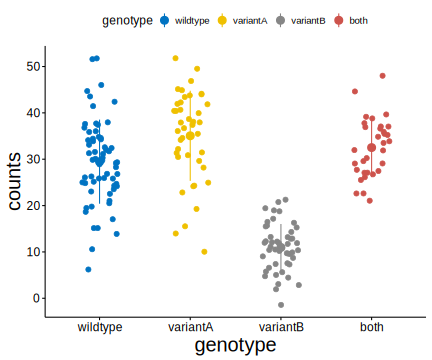
\includegraphics[width=0.8\columnwidth]{./Figures/genetic_interaction_concept.pdf}
	\caption{\textbf{Genetic interaction on transcriptome level:} Counts (expression) of a certain gene depend on the sample's genotype. In variant A the gene is similar expressed as in wildtype samples, whereas variant B clearly inhibits expression. If both variants co-occur this inhibition is reversed. Variant A either blocks the inhibitory effect of variant B or restores the expression by activation of an alternative pathway. By simple combination of the individual effects we would expect a phenotype similar to the one in variant B, thus both variants interact.}
	\label{fig:geneticInteraction}
\end{figure}

\FloatBarrier

\subsection{Gene expression in CLL}
The main challenge of gene expression profiling in CLL is the high heterogeneity. Many different clinical phenotypes varying in tumor progression and prognosis have been described. At the same time a high and growing number of genetic alterations in different combinations are found \citep{Landau2015}. This variety is also reflected on gene expression level and is one reason why only a few distinct associations between gene expression and CLL genotypes have been discovered so far. As consequence, a previous study with 121 CLL patients by \citet{Ecker2015} used gene expression variability instead of actual gene expression level to identify differentially regulated genes. Another study by \citet{Ferreira2014} identified two new subgroups based on transcriptome profiles in 98 CLL patients with stronger signatures than genotype associations. A later study associated these signatures with a technical blood sample processing signature, revealing technical noise as another bottleneck of transcriptome analysis in CLL \citep{Dvinge2014}. The PACE dataset contains the largest transcriptomic profiling dataset for CLL so far and also includes a variety of multi-omics datasets as well as clinical annotations, which provides us a powerful tool to further examine previous hypothesis and gain novel insights on the complex networks among genomic variation, transcription and phenotypes.











\cleardoublepage


%%%%%%%%%%%%%%%%%%%%%%%% Material and Methods %%%%%%%%%%%%%%%%%%%%%%%%%%%%%%%%

\section{Material and Methods}

\subsection{Data}
All data used in this study are part of the Primary Blood Cancer Cell Encyclopedia (PACE) \citep{Dietrich}. Transcriptome data were analyzed starting from unprocessed raw RNA-seq reads. Other data used in this study are patient metadata, classification of methylation groups, drug response groups, FISH data and WGS sequencing data on gene mutations and CNVs. They were received as processed data as available in PACE. The CLL cohort is the largest subgroup within PACE. Genotype data reveal 89 different single gene mutations and CNVs in CLL patients. This study includes genetic variants with a prevalence of more than 3.5\% to ensure statistical power.

\subsubsection{RNA-sequencing}
Trancriptome data of PACE have been generated over a period of 4 years. RNA isolation and library preparation were performed standardized as described in \citet{Dietrich}. In short, total RNA was isolated from patient blood samples using the RNA RNeasy mini kit (Qiagen). For quantification a Qubit 2.0 Fluorometer was used and RNA integrity was evaluated by an Agilent 2100 Bioanalyzer. Thereby samples with a RNA integrity number (RIN) $< 8$ were excluded from the study. Library preparation was performed according to the Illumina TruSeq RNA sample preparation v2 protocol. 
Samples were paired-end sequenced at the DKFZ Genomics and Proteomics Core Facility. 2-3 samples were multiplexed per lane on Illumina HiSeq 2000, Illumina HiSeq3000/4000 or Illumina HiSeqX machines. Platform changes were due to technological development during the period of sequencing and came with changes in read length (101 base pairs (bp), 125 bp and 150 bp) and read number.  

\subsection{Data processing}

\subsubsection{Raw data}
Raw RNA-seq reads were demultiplexed and quality control was performed using FastQC version 0.11.5 \citep{Andrews}. Internal trimming of STAR version 2.5.2a \citep{Dobin2015} was used to remove adapters before mapping \citep{Dobin2015}.

\subsubsection{Alignment}
Mapping was performed using STAR version 2.5.2a \citep{Dobin2015} against the Ensembl human reference genome release 75 (Homo sapiens GRCh37.75) \citep{Flicek2014}. STAR was run in default mode with internal adapter trimming using the $clip3pAdapterSeq$ option. Mapped reads were summarized into counts using Htseq-count version 0.9.0 \citep{Anders2010} with default parameters and $union$ mode. So only fragments unambiguously overlapping with one gene were summarized \citep{Anders2010}.       

\subsubsection{Statistical analysis}
All statistical analyses were performed using R version 3.4. PCAs were generated with the R function $prcomp$. For hierarchical clustering complexHeatmaps package \citep{Gu2016} with euclidean distance as calculated by the R $dist$ function was used. Genes were filtered by variance. Only the 5000 most variant genes were included. Co-occurrence of genetic variants was determined by chi-squared test using $chisq.test$ function of R stats package \citep{RCoreTeam2017}. Associations between principal components and occurrence of genetic variants were determined by student’s t-test using $t.test$ function of R stats package \citep{RCoreTeam2017}. In order to apply multiple testing adjustment considering co-occurrence pattern independent hypothesis weighting (IHW) was used \citep{Ignatiadis2016}. Overall variance of occurrence of genetic variants was applied as covariate. Due to the limited number of tests, IHW resulted in one bin with uniform weights and was reduced to Benjamini Hochberg with false discovery rate (FDR) < 0.1 \citep{Benjamini}.

\subsubsection{Accounting for T-cell contamination}
In order to avoid technical bias, sample contamination with T cells was determined and integrated as co-variable into the gene model for differential expression analysis. The T cell signature was inferred as continuous variable reflecting the amount of contamination. As T cell signature marker genes CD4, CD8A, CD8B, CD3B, CD3G, CD2, CD3E were used. To get a gradient of this signature PCA based on marker gene expression was performed. Rotated data by PC1 loadings were used to display the amount of T cell contamination.  

\subsection{Systematic gene Expression Profiling}

\subsubsection{Differential Expression Analysis}
Differentially expressed genes between samples from different genetic variants were analyzed using DESeq2 version 1.16.1 \citep{Love2014}. Confounding factors identified by EDA were defined in the DESeq2 design matrix and so used as covariate for the GLMs. To account for multiple testing the method of Benjamini and Hochberg, with FDR = 0.1~\citep{Benjamini} was applied.   

\subsubsection{Gene Set Enrichment analysis}
Gene set enrichment was performed using the Bioconductor R package piano version 1.18.0 \citep{Varemo}. Enrichment was tested by GSEA using gene level statistics from DESeq2. Gene sets were downloaded from MSigDB using the Hallmark and Kegg gene set collections version 4.0 \citep{Liberzon2015, Kanehisa2017}. Significance of gene sets was determined based on a background distribution of sampled genes with 1000 permutations. P values were corrected for multiple testing using the method of Benjamini and Hochberg, with FDR = 0.1~\citep{Benjamini}.


\subsubsection{Multivariate model}
To account for co-occurring variants and their influence on gene expression pattern we compared two models, a multivariate model including all variants and a reduced model without the variant of interest. Using the Likelihood ratio test as test statistic in the $DESeq$ function Bioconductor R package DESeq2 version 1.16.1 we tested for differences in gene expression related to the variant of interest controlling for all other variants \citep{Love2014}. We performed multiple testing correction according to Benjamini and Hochberg, with FDR = 0.1~\citep{Benjamini} and filtered for significant results with $\text{p}_\text{adj} < 0.01$.

\subsubsection{Tumor epistasis model}
Gene interaction was modeled by an epistasis model describing observed gene expression by a linear combination of the expression in the two interacting variants.
The empirical Bayes estimates and adjusted p values for the probability to observe the gene expression of the PACE data with this epistasis model was calculated by the $eBayes$ function of the R/Bioconductor package limma \citep{Ritchie2015}. A directionality score for each gene was calculated as described in \citet{Fischer2015}. For genes with a significant p value in the epistasis model the observed expression was modeled depending on a linear combination of the present genetic variants. If the fraction of the variance explained by one variant was above a threshold  determined by the 90\% quantile of all samples and the fraction of the other variant below a threshold determined by the 10\% quantile, the direction of interaction was considered as from the first variant to the second. In order to calculate the fractions of variance one way analysis of variance (ANOVA) was applied using the $anova$ function from the R core package stats \citep{RCoreTeam2017}.




\cleardoublepage


%%%%%%%%%%%%%%%%%%%%% Results %%%%%%%%%%%%%%%%%%%%%%%%%%%%%%%%%%%

\section{Results}

\subsection{Transcriptome data in the Primary blood Cancer Cell encyclopedia (PACE)} 

\subsubsection{Occurence of genetic variants}
PACE includes transcriptome data from 184 CLL patients. In total PACE covers 89 single genetic variants composed of 68 gene mutations and 21 CNVs. Many samples showed multiple variants, which is in line with previous characterization of CLL \citep{Landau2015}. In this study we focused on the most common variants with a prevalence of $> 3.5\%$ resulting in 6 CNVs and 7 gene mutations. Del13q14 was the most common variant with 113 cases. 79 samples were hypermutated in the IGHV gene and 96 had an unmutated IGHV locus. Trisomy12 and TP53 appeared in 23 resp.\ 30 samples.  Figure \ref{fig:tableOverview} shows the occurrence of genetic variants dependent on the sample's IGHV status indicating correlations and anti-correlations between variants. $\chi^2$-squared tests revealed significantly high or low co-occurrence of 8 variant pairs. We found TP53 and Del17p13 highly correlated, as well as Del8p12 and Gain8q24, which are both located on chromosome 8. Hypermutated IGHV was associated with Del11q22.3 and TP53, while Trisomy12 was exclusive for Del13q14 (Figure~\ref{fig:corplot_Chisquare}). 

%\begin{figure}
%	\centering
%	\def\svgwidth{\columnwidth}
%	\input{./Figures/data_overview.pdf_tex}
%	\caption{\textbf{Overview Genetic variants in PACE:} Distribution of the most common genetic variants in the 184 CLL patients included in the PACE transcriptome data set. 6 genetic abberations and 7 gene mutations were have a prevalence of $> 3.5\%$.}
%	\label{fig:Overview}
%\end{figure}       


\begin{figure}
	\centering
	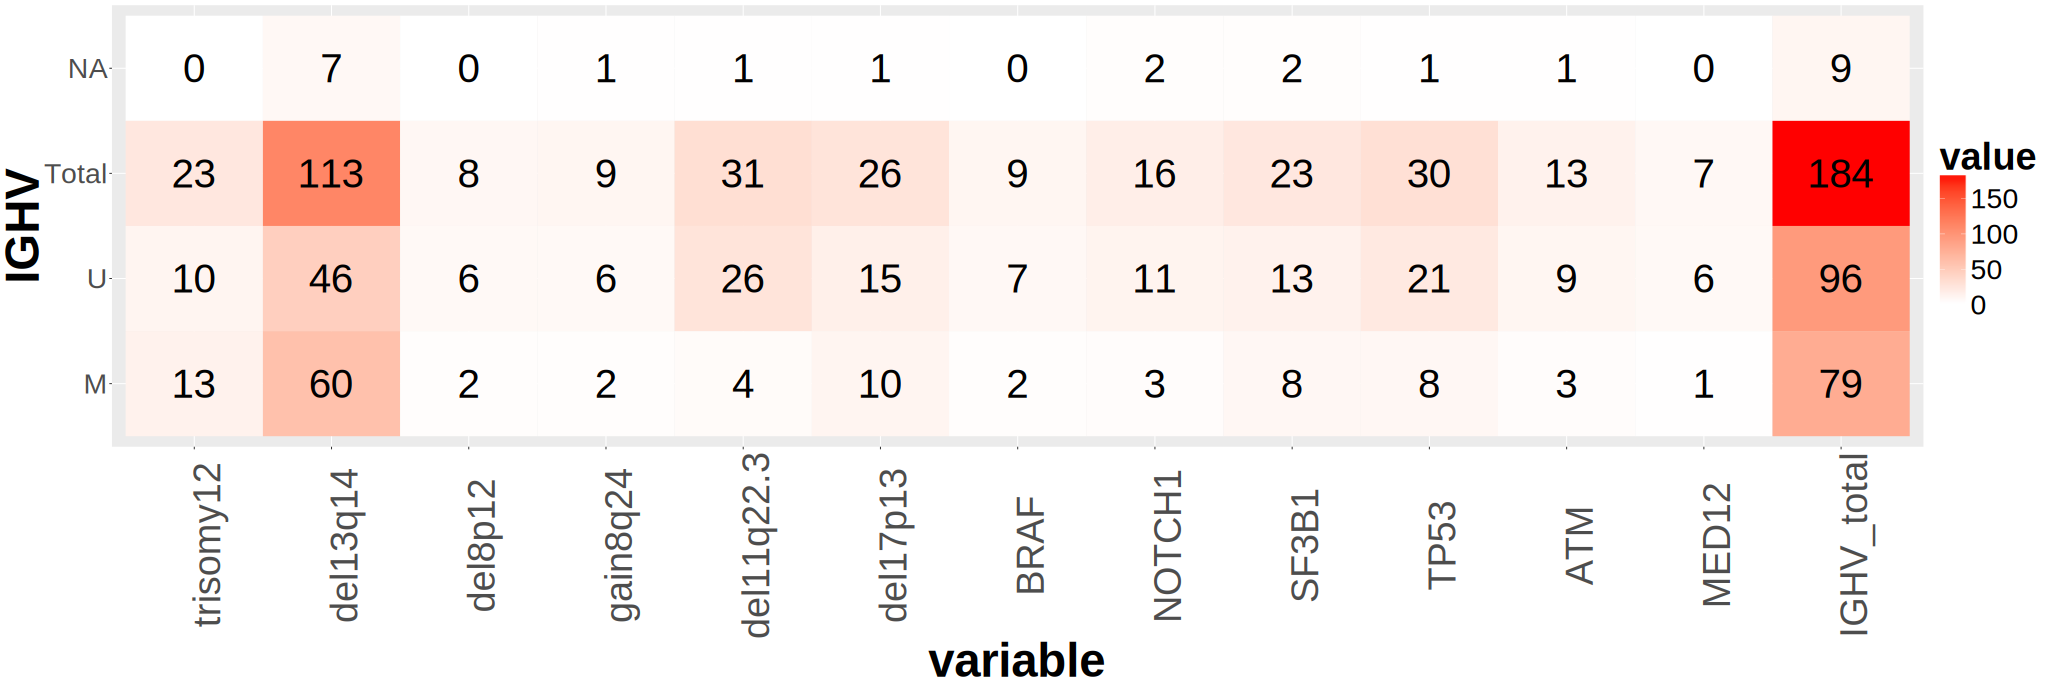
\includegraphics[width=\columnwidth]{./Figures/datatable_overview.pdf}
	\caption{\textbf{Variants in PACE samples by IGHV status:} Most common genetic variants in CLL samples from the PACE transcriptome data set. The distribution by IGHV status for each variant differs, revealing biases and interactivity between variants.}
	\label{fig:tableOverview}
\end{figure}
         

\begin{figure}
	\centering
	\def\svgwidth{\columnwidth}
	\input{./Figures/corplot_chiquare.pdf_tex}
	\caption{\textbf{Co-occurrence of genetic variants:} -log10(pvalue) for co-occurrence of genetic variants calculated by $\chi^2$-square test. The sign indicates the direction of association. Del17p13 and TP53, Del8p12 and Gain8q24, as well as Del11q22.3 and IGHV and Trisomy12 and Del13q14 are significantly associated or excluding.}
	\label{fig:corplot_Chisquare}
\end{figure} 

\FloatBarrier

\subsubsection{IGHV status and Trisomy12 form distinct gene expression cluster}
Genetic profiling of CLL unraveled a variety of driver mutations and genomic features in relation to the disease's phenotypes. Here we aimed to study characteristics of these genetic profiles on transcriptome level. First, we determined the influence of genetic variation on gene expression and thus the capability of PACE to identify specific expression signatures. Hierarchical clustering by the 5000 most variant genes separated samples first by their IGHV status. Samples were further subdivided into the three methylation cluster, which had been classified on the basis of methylome data. Within IGHV groups the Trisomy12 formed sub cluster also revealed a distinct expression pattern. Other variants as TP53, Del11q22.3 and Del13q14 were less connected, but formed several sub cluster with some independent samples. Altogether, clustering revealed an overlap on transcriptome level within different samples based on gene variants (Figure \ref{fig:cluster500exprGenes}).

\begin{figure}
	\centering
	\def\svgwidth{\columnwidth}
	\input{./Figures/cluster500exprgenes.pdf_tex}
	\caption{\textbf{Hierarchical clustering of CLL samples based on the 5000 most variable genes:} Unsupervised sample clustering based on the 5000 most variable genes reveals distinct cluster separated by IGHV status, Methylation groups and Trisomy12.}
	\label{fig:cluster500exprGenes}
\end{figure}


\FloatBarrier

\subsubsection{RNA preparation method, IGHV status and Trisomy12 explain major parts of gene expression variance}

We performed principal component analysis (PCA) to asses to which extend genetic features contribute to the variance of gene expression data. T-test for associations between genetic variants and principal components revealed IGHV status, Trisomy12 and RNA preparation method as main factors to explain genetic variance (Figure \ref{fig:corplot_pca_variants}). Other variants like TP53, Del13q14 and Del11q22 also showed significant associations with one of the first principal components, but correlation and anti-correlation of variants confounded detailed evaluation (see Occurrence of genetic variants). The first principal component (PC1) was associated with the RNA preparation method (Figure \ref{fig:pca}A). Probes collected from a pellet were separated from those extracted by CD19+ selection. CD19 is a B cell marker and selection by CD19+ cells should reduce contamination with other cell types as T cells \citep{Abbasi-Kenarsari2015}. Contamination with other cell types is a common problem in blood cancer samples and we corrected for this as confounding factor in further analyses (see T-cell contamination). 
In line with hierarchical clustering, the second principal component (PC2) displayed IGHV and methylation status, as both are highly correlated (Figure \ref{fig:pca}B/C). Trisomy12 was associated with PC3 and PC4, which still represented 6.2\% and 4.2 \% of the variance (Figure \ref{fig:pca}D). Later principal components like PC9 and PC10 were significantly associated with MED12 and Del17p13, but accounted for less than 2\% of the variance.
Beside their function for quality control these findings validate the suitability of PACE to analyze transcriptional profiles.  

\begin{figure}
	\centering
	\def\svgwidth{\columnwidth}
	\input{./Figures/corplot_pca_variants.pdf_tex}
	\caption{\textbf{Association of genetic variants and principal components:} -log10 (pvalue) t-test for correlation between genetic variants and principal components. PC1 was found to be associated with RNA preparation method and PC2 with IGHV and Del11q22.3. PC3 and PC4 show both significant correlation with Trisomy12 status.}
	\label{fig:corplot_pca_variants}
\end{figure} 

\begin{figure}
	\centering
	\begin{subfigure}[t]{0.45\columnwidth}
		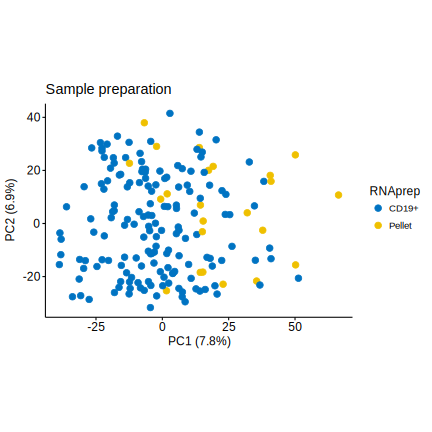
\includegraphics[width=\columnwidth]{./Figures/pca_RNAprep.pdf}
		%\input{./Figures/pca_RNAprep.pdf_tex}
		\subcaption*{}
		\label{fig:pca_RNAprep}
	\end{subfigure}
	\quad
	%add desired spacing between images, e. g. ~,def\svgwidth{\columnwidth} \quad, \qquad, \hfill etc. 
	%(or a blank line to force the subfigure onto a new line)
	\begin{subfigure}[t]{0.45\columnwidth}
		%\def\svgwidth{\columnwidth}
		\includegraphics[width=\columnwidth]{./Figures/pca_ighv_test.pdf}
		%\input{./Figures/pca_ighv.pdf_tex}
		\subcaption*{}
		\label{fig:pca_IGHV}
	\end{subfigure}
	\quad
	\begin{subfigure}[t]{0.45\columnwidth}
		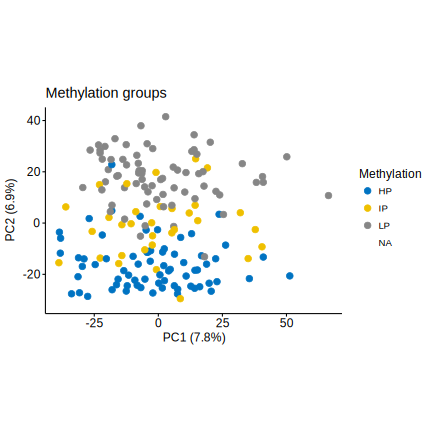
\includegraphics[width=\columnwidth]{./Figures/pca_Methylation.pdf}
		\subcaption*{}
		\label{fig:pca_Methylation}
	\end{subfigure}
	\quad
	\begin{subfigure}[b]{0.45\columnwidth}
		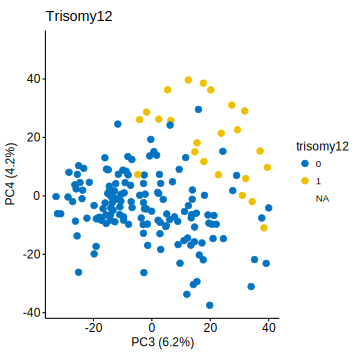
\includegraphics[width=0.8\columnwidth]{./Figures/pca_trisomy12.pdf}
		\subcaption*{}
		\label{fig:pca_trisomy12}
	\end{subfigure}
	\caption{\textbf{Principal component analysis by 5000 most variant genes:} \textbf{(A)} PC1 reflect highest variability within PACE cohort. It correlates with RNA preparation method, which reflects the degree of T-cell contamination. \textbf{(B)} IGHV status is associated with PC2. \textbf{(C)} Methylation groups further refine IGHV distinction. \textbf{(D)} Trisomy12 sample cluster on PC3 and PC4 }
	\label{fig:pca}
\end{figure}


\FloatBarrier

\subsubsection{Confounding factors}

\subsubsection{Batch effects by adapter contamination}
Transcriptome data in PACE were collected over a period of more than four years. During this time sequencing machines and platform were changed enabling to sequence longer reads. These changes in read length were reflected in distinct sample clustering in exploratory data analysis (Figure \ref{fig:Trimming}A). Cluster also correlated with the library adapter contamination. Longer reads showed an increased number of adapters as shown in Figure \ref{fig:adapter_contam}. As insert size distribution of sequenced reads was equal among samples, but read length increased with platform changes, the probability of sequencing into the adapter sequence increased as well. Adapter sequences can infer mapping biases or even lead to mismapping \citep{Sturm}. Thus, adapters were trimmed before mapping, removing the batch effect (Figure \ref{fig:Trimming}B).   

\begin{figure}
	\centering
	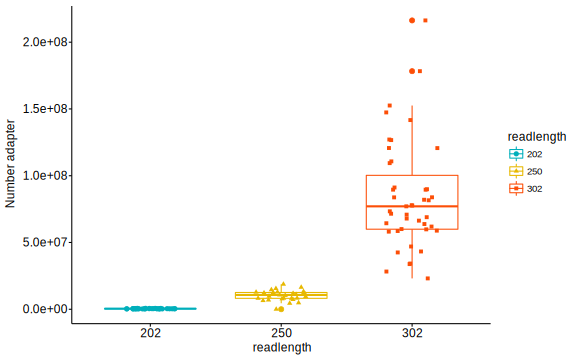
\includegraphics[width=\columnwidth]{./Figures/adapter_contam.pdf}
	\caption{\textbf{Number of detected adapter sequences by length of RNAseq reads:} Total numbers and variance of adapter contamination increases drastic with longer reads. This emphasizes the importance of adapter trimming for reads close to the average length of inserts.}
	\label{fig:adapter_contam}
\end{figure}



\begin{figure}
	\centering
	\begin{subfigure}[t]{0.55\columnwidth}
		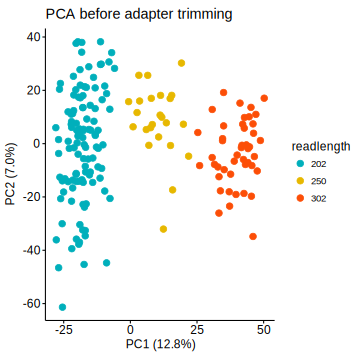
\includegraphics[width=\columnwidth]{./Figures/pca_readlengthOld.pdf}
		\subcaption*{}
		\label{fig:PCA_readlengthOld}
	\end{subfigure}
	\quad
	%add desired spacing between images, e. g. ~,def\svgwidth{\columnwidth} \quad, \qquad, \hfill etc. 
	%(or a blank line to force the subfigure onto a new line)
	\begin{subfigure}[t]{0.6\columnwidth}
		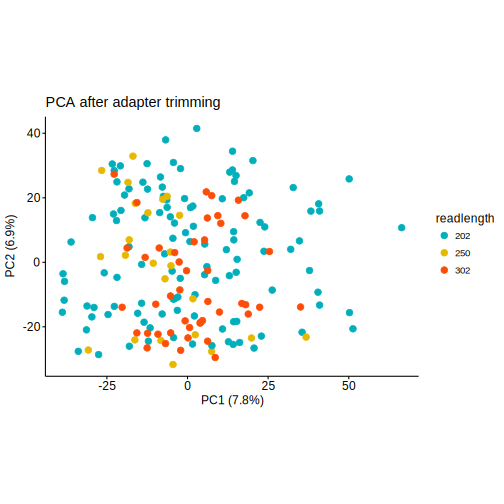
\includegraphics[width=\columnwidth]{./Figures/pca_readlengthtrimmed.pdf}
		\subcaption*{}
		\label{fig:PCA_readlength_trimmed}
	\end{subfigure}
	\caption{\textbf{PCA before and after adapter trimming:} \textbf{(A)} PCA before adapter trimming: The highest variance is associated with the length of RNAseq reads. \textbf{(B)} PCA after adapter trimming: Samples can not longer be distinguished by read length.}
	\label{fig:Trimming}
\end{figure}



\FloatBarrier

\subsubsection{T-cell contamination}
According to exploratory data analysis 7.8\% of variance in PACE transcriptome data were associated to the RNA preparation protocol, which differs in its specificity for B cell selection. To correct for contamination with T cells a variable describing the amount of contamination per sample was introduced and used as co-variable in further gene expression models. T cell marker gene expression showed a gradient between samples, with uniform expression within each sample (Figure \ref{fig:TCell}A). PCA on this marker genes separated sample on PC1 in line with this gradient (Figure \ref{fig:TCell}B). Loadings on PC1 were used to describe the variance of the data set due to T cell contamination.   

\FloatBarrier

\begin{figure}
	\centering
	\begin{subfigure}[t]{\columnwidth}
		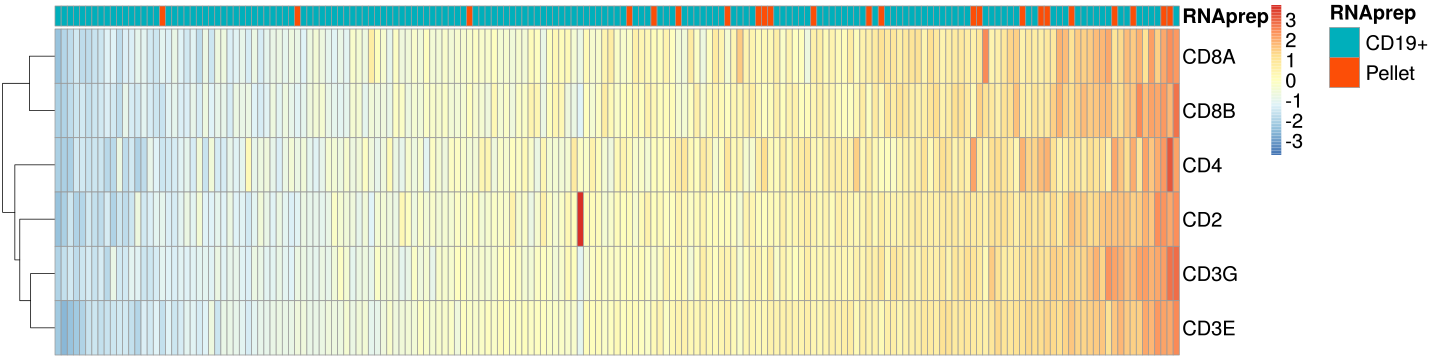
\includegraphics[width=\columnwidth]{./Figures/TmarkExpression.pdf}
		\subcaption*{}
		\label{fig:TmarkExpression}
	\end{subfigure}
	\hfill
	%add desired spacing between images, e. g. ~,def\svgwidth{\columnwidth} \quad, \qquad, \hfill etc. 
	%(or a blank line to force the subfigure onto a new line)
	\begin{subfigure}[t]{\columnwidth}
		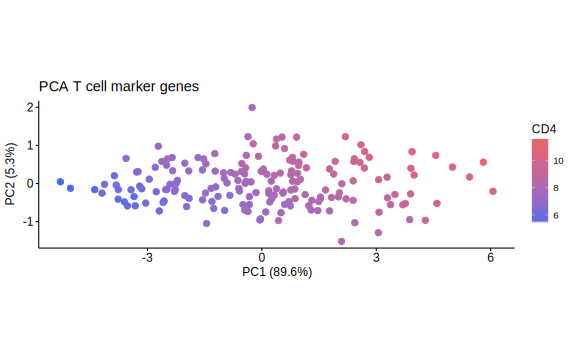
\includegraphics[width=\columnwidth]{./Figures/Tmark_pca.pdf}
		\subcaption*{}
		\label{fig:TmarkPCA}
	\end{subfigure}
	\caption{\textbf{Degree of T cell contamination by marker genes:} \textbf{(A)} T cell marker gene expression show a gradient between samples, with uniform expression within each sample. \textbf{(B)} PC1 describes variance by marker gene expression. Thus loadings were used to quantify T cell contamination.}
	\label{fig:TCell}
\end{figure}

\FloatBarrier



\subsection{Systematic gene Expression Profiling}
Transciptional signatures consist of genes distinguishing variants and were described by differential expressed genes and pathways, that were enriched for them. By integration of other data types and biological knowledge these pattern led to candidates and hypothesis for further investigation.  


\subsubsection{IGHV}
IGHV mutational status is a dominant feature in EDA and resulted in 3873 significant differential expressed genes ($\text{p}_\text{adj} < 0.01$). 92 of them show a $\log_2$ fold change $>4$. These genes could be divided into two groups: those with increased expression in the IGHV-mutated group and those with increased expression in the IGHV-unmutated group, except for Trisomy12 samples. Trisomy12 samples formed a distinct cluster close to the IGHV-mutated cluster. This is internally separated by IGHV status, again indicating interactions between these variants (see Tumor epistatsis). 
In accordance with EDA, methylation groups also clustered by genes distinguishing IGHV groups. Thereby the intermediate group formed a distinct cluster close to the highly methylated group (Figure \ref{fig:gene_exprIGHV_gsea_hallmark}). Marker genes like ZAP-70 and CD38 were higher expressed in IGHV-unmutated samples confirming prior findings. Furthermore SAGE1, which belongs to a class of genes only activated in tumor cells was found in IGHV-unmutated samples. Tumor supressor genes like TP63, TEAD1 and DIRAS3 were also significantly higher expressed. Gene set enrichment analysis revealed B cell receptor signaling as one of the most distinctive changes upon IGHV mutation (Supplements Figure \ref{fig:Enrichment_others}). Using the hallmark gene set annotation revealed a decreased expression of TNF alpha signaling via the NFKB, PI3K-AKT-MTOR pathway and Notch signaling in IGHV-M samples (Figure \ref{fig:EnrichmentTri12IGHV}).  

\FloatBarrier

\begin{figure}
	\centering
	\includegraphics[width=\columnwidth]{./Figures/gene_exprIGHV_gsea_Hallmark.pdf}
	\caption{\textbf{Gene expression of differentially expressed genes by IGHV status:} Samples form distinct cluster depending on IGHV status with Trisomy12 samples forming an own cluster. Genes with $>$ 4.5 $\log_2$ fold change are annotated. Among them are SEPT10, TP63 and TEAD1. Clinical marker ZAP70 and CD38 are up regulated in IGHV unmutated samples.}
	\label{fig:gene_exprIGHV_gsea_hallmark}
\end{figure}


\FloatBarrier

\subsubsection{Trisomy12} 
Trisomy12 is a common genetic variant in CLL samples. On gene expression level we found 3942 differentially expressed genes ($\text{p}_\text{adj} < 0.01$), which formed two major cluster of up and down regulated genes in Trisomy 12 (Figure \ref{fig:gene_exprTriisomy12_gsea_hallmark}). In line with expectations most up regulated genes ($\sim22\%$) were located on chromosome 12 (Figure \ref{fig:tri12_chrom}). Among up regulated genes, we found surface integrins like ITGAM, ITGB2, ITGB1 and ITGB7 and integrin signaling molecules associated with VLA-4 directed adhesion. Similar to the IGHV unmutated group, up regulated genes were enriched in TNF alpha signaling via NFKB, PI3K-AKT-MTOR signaling, Notch signaling and P53. In contrast, down regulated genes were associated with bile acid metabolism and glycolysis (Figure \ref{fig:EnrichmentTri12IGHV}B). 

\FloatBarrier

\begin{figure}
	\centering
	\includegraphics[width=\columnwidth]{./Figures/gene_exprTrisomy12_gsea_Hallmark.pdf}
	\caption{\textbf{Gene expression in Trisomy12:} Trisomy12 samples form a separate cluster with distinct gene expression. Genes with $\log_2$ fold changes $>4.5$ are annotated. Among them surface integrins like ITGAM, ITGB2, ITGB1 and ITGB7 can be found. Many up regulated genes are located on chromosome 12.}
	\label{fig:gene_exprTriisomy12_gsea_hallmark}
\end{figure}


\begin{figure}
	\centering
	\begin{subfigure}[t]{0.48\columnwidth}
		\includegraphics[width=\columnwidth]{./Figures/chromosom_dist_up.pdf}
		\subcaption*{}
		\label{fig:tri12_chrom_dn}
	\end{subfigure}
	\hfill
	%add desired spacing between images, e. g. ~,def\svgwidth{\columnwidth} \quad, \qquad, \hfill etc. 
	%(or a blank line to force the subfigure onto a new line)
	\begin{subfigure}[t]{0.48\columnwidth}
		\includegraphics[width=\columnwidth]{./Figures/chromosom_dist_down.pdf}
		\subcaption*{}
		\label{fig:tri12_chrom_up}
	\end{subfigure}
	\caption{\textbf{Chromosomal distribution of genes differentially expressed in Trisomy12 samples:} \textbf{(A)} 22\% of up regulated genes are located on chromosome 12. Numbers in captions indicate the number of differentially expressed genes located at this chromosome. \textbf{(B)} 
		Genes down regulated in Trisomy12 samples are approximately equally distributed among chromosomes.}
	\label{fig:tri12_chrom}
\end{figure}


\begin{figure}
	\centering
	\begin{subfigure}[t]{0.48\columnwidth}
		\includegraphics[width=\columnwidth]{./Figures/gsea_IGHV.pdf}
		\subcaption*{}
		\label{fig:gsea_IGHV}
	\end{subfigure}
	\hfill
	%add desired spacing between images, e. g. ~,def\svgwidth{\columnwidth} \quad, \qquad, \hfill etc. 
	%(or a blank line to force the subfigure onto a new line)
	\begin{subfigure}[t]{0.48\columnwidth}
		\includegraphics[width=\columnwidth]{./Figures/gseaHallmark_trisomy12.pdf}
		\subcaption*{}
		\label{fig:gsea_trisomy12}
	\end{subfigure}
	\caption{\textbf{Enriched hallmark gene sets:} \textbf{(A)} Enriched pathways in IGHV samples are shown. Up regulated pathway as angiogenesis are higher expressed in IGHV-mutated samples. Down regulated pathways in IGHV mutated vs unmutated samples are TNF alpha signaling via NFKB and PI3 MAP Kinase pathway. \textbf{(B)} Trisomy12 activates many pathways like TNFA via NFKP, Notch pathway and PI3 MAP Kinase pathway.}
	\label{fig:EnrichmentTri12IGHV}
\end{figure}

\FloatBarrier


\subsubsection{TP53 and Del17p53}
The TP53 gene is located at the locus of Del17p13. Thus TP53 mutation in combination with Del17p13 lead to a homozygote loss of function for TP53, which is a regulator of DNA damage response. More than half of all samples with Del17p13 were found to have a mutated TP53 gene at the other allel. Gene signatures of mutation and deletion were dominated by down regulated genes on chromosome 17 (Figure \ref{fig:gene_exprdel17p13_gsea_kegg}). Patterns of up regulated genes were less distinct. All in all 929 genes were differentially expressed in Del17p13 samples and 474 in TP53 samples ($\text{p}_\text{adj} < 0.01$). Half of those were overlapping with Del17p13 (Figure \ref{fig:GeneDist17}). TP53 itself was down regulated and clustered with other genes on chromosome 17. Most of Del17p13 and TP53 samples formed one distinct cluster with a correlated expression signature. A few samples showed distinct differences in gene expression, even for down regulated genes on chromosome 17. They seemed to be dominated by another mechanism independent of TP53 and genes on chromosome 17. Enrichment tests revealed DNA repair pathway down regulated in TP53 samples. This is in line with the function of TP53 for DNA damage control. Furthermore both variants are associated with down regulation in Wnt Beta Catenin signaling.   

\FloatBarrier

\begin{figure}
	\centering
	\includegraphics[width=\columnwidth]{./Figures/gene_exprDel17p13_gsea_Kegg.pdf}
	\caption{\textbf{Gene expression in Del17p13 and TP53:} Del17p13 samples cluster together with a few exceptions. Most of these exceptions do not show a TP53 mutation and thus not a complete loss of TP53 function. The cluster is driven by down regulated genes (most located on chromosome 17) including TP53.}
	\label{fig:gene_exprdel17p13_gsea_kegg}
\end{figure}

\begin{figure}
	\centering
	\begin{subfigure}[t]{0.8\columnwidth}
		\includegraphics[width=\columnwidth]{./Figures/chromosom17_dist_down.pdf}
		\subcaption*{}
		\label{fig:chromosom17_dist_down}
	\end{subfigure}
	\quad
	%add desired spacing between images, e. g. ~,def\svgwidth{\columnwidth} \quad, \qquad, \hfill etc. 
	%(or a blank line to force the subfigure onto a new line)
	\begin{subfigure}[t]{0.6\columnwidth}
		\includegraphics[width=\columnwidth]{./Figures/vennDel17TP53.pdf}
		\subcaption*{}
		\label{fig:vennDel17TP53}
	\end{subfigure}
	\caption{\textbf{Distribution of differentially expressed genes in TP53 and Del17p13} \textbf{(A)} More than half of all down regulated genes in Del17p13 samples are located on chromosome 17. Numbers in captions indicate the number of differentially expressed genes located at this chromosome. \textbf{(B)} There is a high overlap of differentially expressed genes in TP53 and Del17p13.}
	\label{fig:GeneDist17}
\end{figure}


\FloatBarrier

\subsubsection{Del11q22.3 and ATM}
Del11q22.3 is another common deletion in CLL samples. Analysis revealed 430 significantly differential expressed genes ($\text{p}_\text{adj} < 0.05$). About half of them were down regulated and 30.5\% were located on chromosome 11. With some exception Del11.22.3 samples formed a distinct cluster with common gene expression pattern of down regulated as well as up regulated genes (Figure \ref{fig:gene_exprdel11q22.3_gsea_hallmark}). Up regulated pathways were myogenisis, Myc targets and heme metabolism, whereas protein secretion and mitotic spindle were down regulated (see supplements Figure \ref{fig:Enrichment_others}B). The ATM gene is localized on chromosome 11q22 and more than half of all samples with ATM mutation (13 cases in total) had a deletion on the second chromosome. A specific signature for ATM mutation alone or for homozygotic ATM loss of function was not identified, but ATM was among differentially down regulated genes in Del11q22 samples.  

\FloatBarrier

\begin{figure}
	\centering
	\includegraphics[width=\columnwidth]{./Figures/gene_exprdel11q22_gsea_Hallmark.pdf}
	\caption{\textbf{Gene expression in Del11q22.3 and ATM:} Del11q22 samples cluster driven by deleted genes on chromosome 11 like ATM. Nevertheless loss of ATM function does not seem to be the only driving factor, but a set of genes including SEPT10 is also up regulated.}
	\label{fig:gene_exprdel11q22.3_gsea_hallmark}
\end{figure}

\FloatBarrier



\subsubsection{Del13q14}
Del13q14 is the most common CNV in PACE. Nonetheless the degree of deletion varies a lot between a loss of 100\% and 0\%. On gene expression level the degree of Del13q14 did not correlate with expression pattern at all (see Supplements Figure \ref{fig:gene_exprdel13q14_gsea_kegg}). No pathways were significantly enriched for differentially expressed genes either. A subgroup of samples showed distinct down regulation of a small set of genes that were located at 13q14, including KPNA3, DLEU1, KCNRG, PHF11. Thereby the subgroup itself could not be distinguished by Del13q14 status. Genes from the minimal deleted region like DLEU2, miR15a/16a and genes regulated by the mir15a-mir16a complex like BCL2 were not differentially expressed. Major tumor progressive effects of Del13q14 does not seem to be displayed at gene expression level. 

\subsubsection{Del8p12 and Gain8q24}
More than half of all samples with Gain8q24 show an earlier deletion Del8p12 as genetic instability on chromosome 8. Thus, Del8p12 and Gain8q24 samples showed both, significantly up- and down regulated genes on chromosome 8. In total 206 resp 285 genes were differentially expressed and enriched in similar pathways (Figure \ref{fig:gene_exprgain8q24_gsea_Hallmark}). Unfolded protein response, mTORC1 signaling and Myc targets were up and myogenesis was significantly down regulated (see Supplements Figure \ref{fig:Enrichment_others}C). Enrichment in Myc targets was in line with prior findings and has been proposed as possible mechanism of Gain8q24 tumorigenesis.

\FloatBarrier

\begin{figure}
	\centering
	\includegraphics[width=\columnwidth]{./Figures/gene_exprgain8q24_gsea_Hallmark.pdf}
	\caption{\textbf{Gene expression in Gain8q24 and Del8p12:} Differentially expressed genes in Gain8q24 sample cluster by Gain8q24 and Del8p12 revealing interaction of these variants. Thus, we find up and down regulated genes on chromosome 8  among differentially expressed genes. Genes with $\log_2$ fold changes $>2$ on chromosome 8 are annnotated.}
	\label{fig:gene_exprgain8q24_gsea_Hallmark}
\end{figure}

\FloatBarrier


\subsubsection{SF3B1}
Samples with SF3B1 mutation formed a distinct cluster based on differentially expressed genes. 311 genes were significantly up regulated and 162 down regulated ($\text{p}_\text{adj} < 0.01$) (Figure \ref{fig:gene_exprSF3B1_gsea_kegg}). These genes were enriched in metabolic pathways as cholesterol homeostasis, as well as interferon alpha signaling, Notch signaling and Myc targets (see Supplements Figure \ref{fig:Enrichment_others}D). Genes like UQCC1 and EBF1 were significantly up regulated in SF3B1 mutated samples.

\FloatBarrier

\begin{figure}
	\centering
	\includegraphics[width=\columnwidth]{./Figures/gene_exprSF3B1_gsea_Hallmark.pdf}
	\caption{\textbf{Gene expression in SF3B1 mutated samples:} Differentially expressed genes in SF3B1 samples form a distinct cluster. SF3B1 mutation is associated with truncated splicing. This leads to coordinated changes on expression level. Genes with $\log_2$ fold change $>4$ are annotated. }
	\label{fig:gene_exprSF3B1_gsea_kegg}
\end{figure}

\FloatBarrier

\subsubsection{BRAF}
Only 3.5\% of PACE samples show a BRAF mutation. Still 678 genes were differentially expressed in this subgroup ($\text{p}_\text{adj} < 0.01$) and BRAF samples formed a distinct cluster. Clear expression pattern were seen in up regulated genes, which were enriched for G2M checkpoint (figure \ref{fig:gene_exprBRAF_gsea_Hallmark}). Down regulated genes did not show consistent pattern among BRAF samples.  

\FloatBarrier

\begin{figure}
	\centering
	\includegraphics[width=\columnwidth]{./Figures/gene_exprBRAF_gsea_Hallmark.pdf}
	\caption{\textbf{Gene expression in samples with mutated BRAF:} Gene expression in BRAF samples does not show overall coherent cluster. Still a set of up regulated genes that mainly consist of G2M checkpoint genes correlates clearly with BRAF status.}
	\label{fig:gene_exprBRAF_gsea_Hallmark}
\end{figure}

\FloatBarrier
\clearpage

\subsubsection{MED12}
Only 7 of 184 samples show mutated MED12 the PACE dataset did only reveal a few distinct differentially expressed genes (see Supplements Figure \ref{fig:gene_exprMED12_gsea_Hallmark}). MED13L was among down regulated genes. It is part of the mediator complex and supports prior findings \citep{Kampjarvi2015}.

\FloatBarrier


\subsubsection{Notch1}
In total Notch1 mutation was found in 16 samples. 162 genes were differentially expressed ($\text{p}_\text{adj} < 0.05$) between them and other samples in PACE. Despite its adverse clinical prognosis we could not identify distinct gene expression pattern or chromosomal distributions within those (see Supplements Figure \ref{fig:gene_exprNOTCH1_gsea_Hallmark}).

\subsection{Multivariate model}
To account for the effect of co-occurring variants on gene expression we used likelihood ratio tests in differential expression analysis. By comparison of a multivariate model including all variants with a reduced model without the variant of interest we tested for differentially expressed genes in each individual variant controlling for all other variants. As we tested for genes that were solely associated to the individual variants, the numbers of differentially expressed genes were clearly reduced. We still found 1012 genes significantly related to Trisomy12 and 414 related to IGHV status, but for all other variants we found less than 90 and for 5 variants even less than 10 differentially expressed genes (Figure\ref{fig:compModel}). Especially for those variants that were functional correlated, including Del17p13 and TP53 and Del11q22 and ATM, only a few genes were exclusively associated to one variant. The top 7 genes that were differentially expressed in the individual variants are shown in Figure \ref{fig:reducedModel}. We found ATM associated to Del11q22, even when controlling for ATM mutations. Still integrins like ITGF2 were significant in Trisomy12 samples and Notch4 was differentially expressed in Notch1 mutated samples. For Del8p12 the only significant result was KIF13B. This gene is located in the deleted region of Del8p12. These findings are in line with previous results and our expectations. Interestingly, RRM2 was among genes differentially expressed in samples with mutated BRAF.     

\FloatBarrier

\begin{figure}
	\centering
	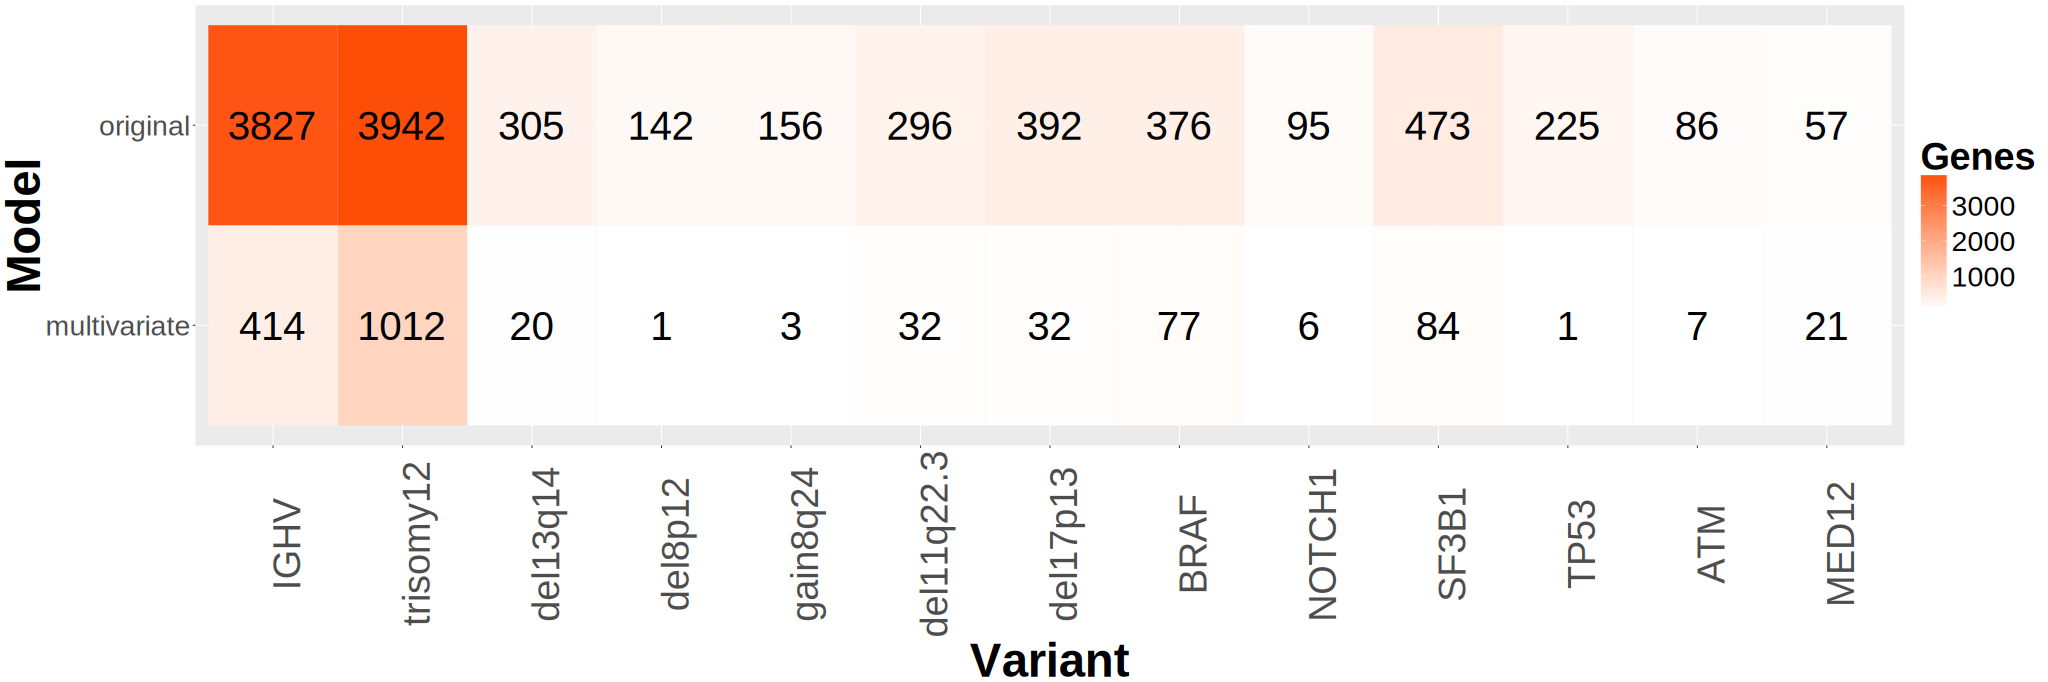
\includegraphics[width=\columnwidth]{./Figures/comparisonModel.pdf}
	\caption{\textbf{Top 7 genes of significant results in the original model and the multivariate model:} For all variants the numbers of differentially expressed genes were clearly reduced when testing for individual variants in a multivariate model against a reduced model by the likelihood ratio test. The original model included IGHV status, Trisomy12 and degree of T cell contamination as covariate. Still 1012 genes are significantly related to Trisomy12 and 414 related to IGHV status, when we control for the effect of confounding variants. Only a few genes are associated to the other variants.}
	\label{fig:compModel}
\end{figure}




\begin{figure}
	\centering
	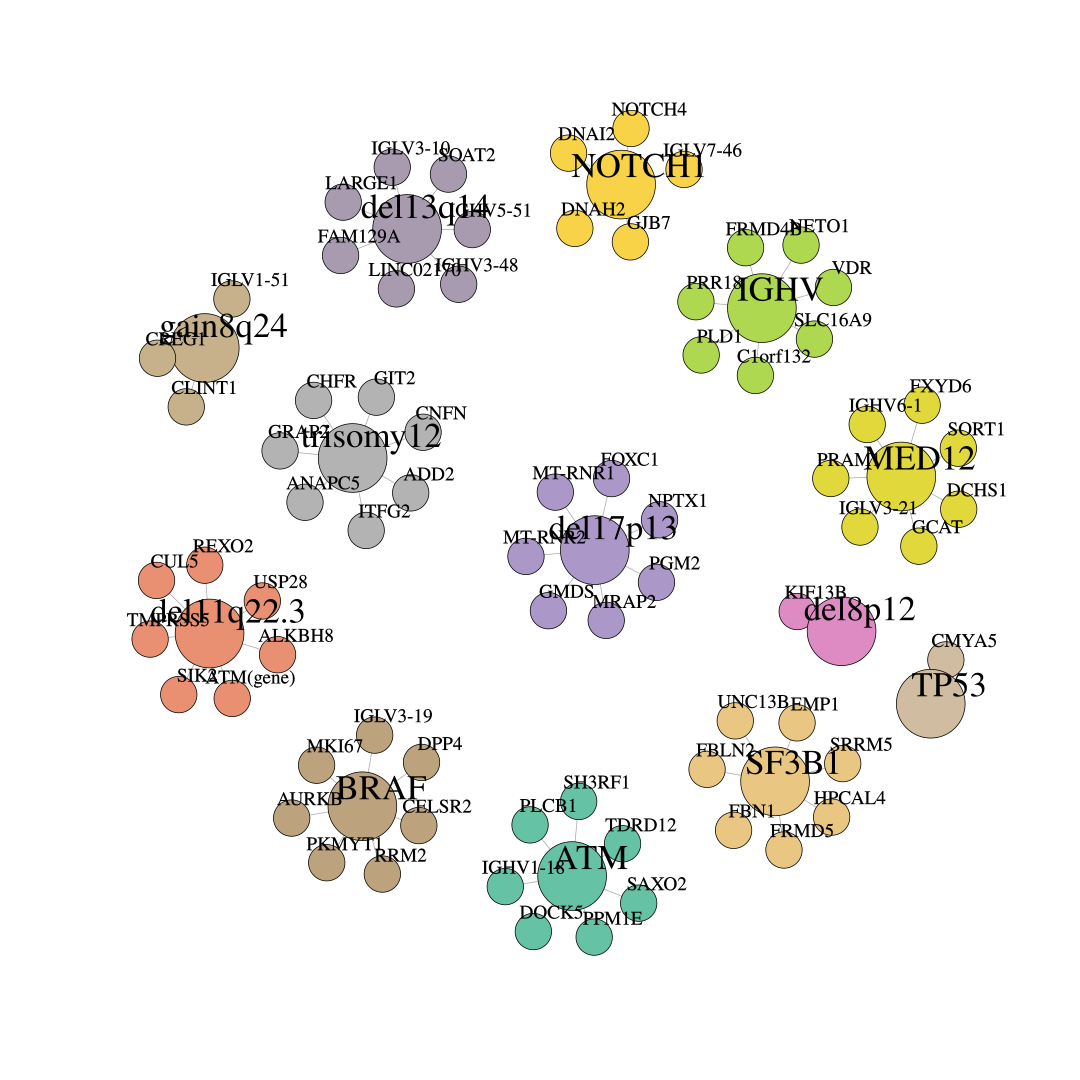
\includegraphics[width=\columnwidth]{./Figures/reducedModel.pdf}
	\caption{\textbf{Most significant differentially expressed genes testing for the effect of each variants alone:} Using a likelihood ratio test to compare a multivariate model with all variants against a reduced model with confounders resulted in small sets of genes related to the individual variants controlling for all other variants. Some of these sets contain less than 7 significant genes. Still we can find known associations like differentially expression of ATM gene in DEL11q22 samples and Notch4 in Notch1 samples.}
	\label{fig:reducedModel}
\end{figure}

\FloatBarrier



\subsection{Methylation profiles in gene expression}
Using the most variant genes, samples formed distinct cluster associated with methylation groups in a PCA (Figure  \ref{fig:pca_Meth_top150}). This indicated an important role of epigenomic regulation in gene expression of CLL. Transcription factor deregulation by differential de-methylation has been suggested as a tumor determining process. EGR1, NFAT and EBF1 were associated with differences in methylation pattern. In line with this, genes of these transcription factors themselves were among genes with highest loadings on PC1, which separated samples by methylation groups. In total 3 out of 4 transcription factors, that have been identified as potentially pathogenic in CLL \citep{Oakes2016}, showed gene expression correlating with methylation groups (Figure \ref{fig:gene_expr_Methylationgroups_top150}). 

\FloatBarrier

\begin{figure}
	\centering
	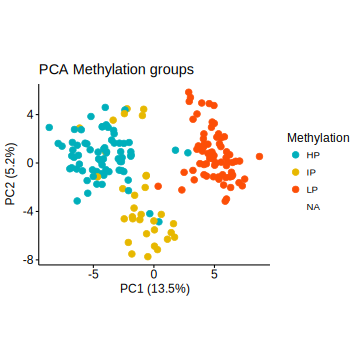
\includegraphics[width=0.75\columnwidth]{./Figures/pca_Meth_top150.pdf}
	\caption{\textbf{Principal component analysis methylation groups:} PC1 and PC2 clearly separate methylation groups into 3 cluster based on expression of the 200 most variable genes.}
	\label{fig:pca_Meth_top150}
\end{figure}


\begin{figure}
	\centering
	\includegraphics[width=\columnwidth]{./Figures/gene_expr_Methylationgroups_top150.pdf}
	\caption{\textbf{Gene expression of the 200 most variable genes:} The 200 most variable genes show distinct expression within each methylation group. Among them are multifunctional transcription factors like EGR1, NFAT and EBF1.}
	\label{fig:gene_expr_Methylationgroups_top150}
\end{figure}

\FloatBarrier

\subsection{Tumor epistasis in IGHV and Trisomy12}

Differential expression analysis revealed distinct gene signatures between IGHV subtypes and Trisomy12 (Figure \ref{fig:gene_exprIGHV_gsea_hallmark}). Trisomy12 samples formed a separate cluster close to the IGHV mutated samples. Inside this cluster, samples grouped again by IGHV status. It is known that the interplay of different genetic variants characterizes tumorigenesis and can determine cancer phenotype and clinical outcome \citep{Landau2015}. We show here, that gene expression data can also reflect this interplay between Trisomy12 and IGHV hypermutations. The combined genotype showed different expression pattern from what would have been expected from the individual effects of the variants. Modeling gene expression as epistatic interaction resulted in 602 significantly associated genes in the presence of IGHV hypermutations and Trisomy12, together or alone (Figure \ref{fig:epistasisTri12IGHV}). They formed 5 cluster with distinct gene expression patterns, suggesting different layer of interactivity. The first cluster represented genes only down regulated in IGHV unmutated samples. A subset of these genes was located on chromosome 12, which could be a reason why down regulation failed in Trisomy12 samples with unmutated IGHV status. Further clusters showed strong up resp. down regulation in CLL-M samples with Trisomy12. These clusters showed clear interaction on gene expression level between Trisomy12 and IGHV. Significantly up-regulated genes were CD38, MAP3K8 and CDCP1. Another gene cluster represented genes up regulated in Trisomy12 samples without IGHV mutations. In the presence of both trisomy12 and IGHV mutation, the up regulation of those genes were suppressed. As described by Fischer et al. [2015], we inferred directions for each gene describing the interactions as one variant alleviating or aggravating the effect of the other. Interestingly, we observed consistent directions within gene clusters. This confirmed our observation, that the clusters represent different layer of interactivity. In the cluster with enhanced expression in M-CLL with Trisomy12 the interaction was directed from IGHV to Trisomy12, whereas in the cluster with genes down regulated in IGHV unmutated samples, the presence of Trisomy12 determined the effect of the IGHV status on gene expression.       


\FloatBarrier

\begin{figure}
	\centering
	\includegraphics[width=\columnwidth]{./Figures/epistatsisTri12IGHV.pdf}
	\caption{\textbf{Genes differentially expressed between samples with Trisomy12, IGHV mutated, both or IGHV-unmutated genotypes:} Genes can be distinguished into 5 groups revealing clear patterns of interactivity. The direction of interaction is consistent within these clusters.}
	\label{fig:epistasisTri12IGHV}
\end{figure}

\FloatBarrier


\cleardoublepage


%%%%%%%%%%%%%%%%%%%%%%%%%%% Discussion %%%%%%%%%%%%%%%%%%%%%%%%%%%%%%%%%%%%%%%%%%%%%

\section{Discussion}


\subsection{Gene expression signatures in CLL}
Due to the phenotypic and genotypic heterogeneity of CLL, gene expression profiling on CLL has yet provided little insight into molecular mechanisms underlying different genotypes.     
The PACE study represents the most comprehensive data set of CLL transcriptomes so far. We were able to distinguish gene expression profiles by the most prevalent genomic variants like IGHV hypermutations and Trisomy12 in an unsupervised approach. Groups classified by methylation pattern were clearly distinguishable by hierarchical clustering as well as PCA of gene expression data. These findings validate the quality of PACE and indicate its potential for detailed gene expression analysis. At the same time, they confirm distinct changes on gene expression level due to IGHV mutations and Trisomy12. We found 6.9\% of gene expression variability associated with IGHV status, in contrast to previous findings of only 1.5\% \citep{Ferreira2014}. This reveals the strength of our data set, due to the large sample size compared to previous studies.    
In total we analyzed gene expression profiles of the 13 most common single genetic variants and found distinct gene expression pattern for 8 of them. Thus, the PACE data set can serve as basis to study underlying molecular mechanisms in detail. 

\subsubsection{B cell receptor signaling is up regulated in IGHV-unmutated samples}
B cell receptor (BCR) signaling plays a decisive role in B cell survival and proliferation. CLL samples with unmutated IGHV genes showed increased activation and usually expressed polyreactive BCRs and high level of CD38 and Zap70, which are established clinical marker. As shown in previous studies IGHV mutated samples express more specific BCRs and show low activation of B cell receptor signaling \citep{Hacken2016}. Our Gene expression data confirmed these findings and we could show that up regulation of BCR signaling, CD38 and Zap70 in IGHV-unmutated samples proceeds already on transcriptome level. Downstream pathways like TNF alpha signaling via NFKB and PI3K-AKT-MTOR signaling were also enriched. Besides, we found the expression of tumor supressor genes, including TP63, TEAD1 and DIRAS3, increased in IGHV unmutated samples. This is in line with a prior finding that BCR signaling down regulates TP63 in CLL and therefore promotes tumor progression \citep{Humphries2013}. This regulation by BCR signaling is less prevalent in IGHV-mutated samples, where we found tumor suppressors down regulated on gene expression level.  


\subsection{Trisomy12 samples show increased expression of integrins driving lymphnode homing}
Even though Trisomy12 is a frequent and drastic chromosomal aberration in CLL the molecular mechanisms driving its pathology are not known. Recent studies found that lymphocyte adhesion cascade resulting in increased lymphnode homing of malignant B cells was activated in Trisomy12 samples \citep{Riches2014,Ganghammer2015}. The CD49d, subunit of VLA-4 is a major driver of the lymphocyte adhesion cascade \citep{Strati2017}. Furthermore the relevance of stimulating factors from the lymph node environment has been shown in many cell culture studies \citep{Hacken2016}. Gene expression data confirmed the up regulation of CD49d, as well as surface integrins ITGAM, ITGB2, ITGB1, ITGB7 and intracellular integrin signaling molecules like RABP-1. These surface integrins facilitate cellular adhesion and promote transendothelial migration of circulating cells into the lymph node. Our results support prior hypothesis that increased lymphonode homing acts as a major mechanism for tumor progression in CLLs with Trisomy12 and further confirm the relevance of the lymph node environment in CLL.         


\subsection{Down regulation of TP53 is associated with Wnt-signaling}
Deletion and mutation of TP53 lead to similar gene expression patterns, which can be associated to DNA damage response and Wnt-signaling. Most samples have a complete loss of functional TP53, but some exhibit only one dysfunctional allele. Those differed often in their gene expression from samples with a complete loss of TP53 function. In contrast to most of the other variants, the mechanism of tumor progression underlying TP53 loss of function is already known and related to its function for DNA damage control. Consistent with this, differentially expressed genes associated with TP53 were enriched in DNA damage response pathway. We further found Wnt/beta-Catenin signaling up regulated by TP53 loss. Deprived Wnt suppression by TP53 has already been observed in other cancers like prostate and colorectal cancer \citep{Kim2011a}. Furthermore, Wnt activation has been associated with amplified Myc activation, which is a known proto-oncogene driving cell proliferation \citep{Rennoll2015}. Remarkably, we also found up regulation of Myc targets on gene expression level. Altogether, those are strong evidence for dysregulated Wnt signaling as consequence of complete functional loss of TP53. This could impact tumor progression in other cancer types in a similar way, but further investigation is needed. One possible way is to investigate the role of mir-34, which is associated with Wnt supression via TP53. But micro-RNA detection in poly-A selected RNA sequencing data is not reliable and thus further experimental examination is necessary.         


\subsection{Del11q22 samples cluster by IGHV status}
Del11q22 samples formed a distinct cluster, characterized by the down regulation of ATM, BIRC2 and other genes on chromosome 11. This cluster correlated with IGHV unmutated status, while IGHV-mutated samples showed different gene expression pattern. Co-occurrence analysis already revealed biases in IGHV status and Del11q22. Furthermore we found marker genes like SEPT10 that had been associated with IGHV status differentially expressed in Del11q22 samples before \citep{Benedetti2007}. Together these results suggest an interaction among those variants, which share similar gene expression regulations and underlying mechanisms. ATM mutation is less frequent than Del11q22 and has been proposed as a later event that is often driven by monoallelic loss of the other ATM gene \citep{Landau2015}. We could not distinguish between mono- or biallelic loss of ATM function on gene expression level and did not find differential expression of genes involved in DNA damage control. This indicates a primary mechanism of Del11q22 in tumor progression independent of ATM driven DNA damage control, with ATM mutation as a later event in tumor manifestation.    

\subsection{Interferon signaling and the chaperone UQCC complex are transcriptional regulated in SF3B1 mutated CLLs}
SF3B1 is a splicing factor and related to aberrant RNA and ribosomal procession. A prior study that investigated transcriptomic regulation by differential exon usage revealed similar pattern as in melanoma samples \citep{Reyes}. They suggest a specific role of UQCC and RPL31 in transcriptional regulation of CLL and melanoma. UQCC is a chaperone involved in cytochrome B biosynthesis, but a specific relation to tumorigenesis has not been discovered yet. Interestingly we found UQCC1 gene differentially up regulated in SF3B1 mutated samples. Furthermore, differentially expressed genes were enriched in interferon alpha response, which is in line with findings from differential exon usage. Altogether this supports a functional role on transcriptional regulation of UQCC and interferon signaling as important mechanisms in SF3B1 mutated CLL samples. Overall we found distinct gene expression pattern. The investigation of isoforms and splice pattern could unravel further effects of transcriptional regulation and complement our findings. Furthermore, expression analysis of UQCC in melanoma could help to reveal its significance for tumor progression, as the common pattern in exon usage suggest similar underlying mechanisms. 

\subsection{Cell cycle progression in G2 phase as a potentially altered pathway in BRAF mutated CLLs}
Gene expression in BRAF mutated CLLs was less distinct compared to other genetic variants. Nevertheless, genes related to G2M checkpoint were coordinately up regulated. BRAF mutations are common in various cancer types and usually activate MAPK signaling via the RAS/RAF, MEK/ERK pathway. A direct role of oncogenic activated MAPK signaling for G2 progression and cell cycle activation has already been shown in thyroid follicular neoplasms and our analysis indicates it as a potential mechanism of tumor promotion in CLL \citep{Knauf2006}.

\subsection{Genome de-methylation defines subgroups of CLL with distinct gene expression pattern}
The degree of de-methylation separates CLL samples into groups of high-, intermediate- and low- programmed genomes. We show that these groups are reflected on transcriptional level with distinct gene expression pattern. Differential de-methylation of a set of multifunctional transcription factors has been proposed as tumor promoting mechanism determining these groups. Remarkably, we find 3 out of 4 transcription factors from this set differentially expressed between methylation groups. These findings support the relevance of methylation groups as well as their pathogenic function by differentially methylated multifunctional transcription factors. 


\subsection{Tumor epistasis in Trisomy12 and IGHV results in distinct expression pattern in line with drug response phenotypes}
A recent study by \citet{Bulian2017} on 951 CLL samples identified IGHV status as the most reliable prognostic marker in Trisomy12 CLLs. Overall survival and time to first treatment differed significantly among those four group of samples: U-CLLs with Trisomy 12, M-CLLs with Trisomy12, U-CLLs without Trisomy12 and M-CLLs without Trisomy12. Our data and analysis provide support for this observation. Trisomy12 samples formed an extra cluster regardless of IGHV status. In a model considering a linear combination of the genotype effects, we found 602 genes with significant epistatic expression pattern in samples with co-occurrence of Trisomy12 and IGHV hypermutations. These genes formed clusters that reflect different ways how the variants interact e.g. alleviating or aggravating another. Using analysis of variance we could infer directions describing the hierarchy of interaction. These directions were consistent within gene cluster, which supports our hypothesis of different layers of interaction between the genetic variants. Particularly, the group of Trisomy12 and IGHV mutated samples showed strong up regulation of a set of genes, including CD38 and MAP3K8(TPL2). A drug response study of the PACE data set found an increased sensitivity of Trisomy12 samples towards MEK/ERK inhibitors \citep{Dietrich}, which was rescued in M-CLLs. TPL2 directly activates ERK1/2 downstream of the usual Ras/Raf cascade as an alternative pathway \citep{Rousseau2016}. Gene expression data suggest increased TPL2 level in M-CLL as dominant activator of ERK as a way how Trisomy12 M-CLLs resist MEK/ERK inhibitors.  

\subsection{A multivariate model controls for confounding by other variants and gives insight into gene regulation with another resolution.}
Differential expression analysis of the effect of each variant solely resulted in strong reduction of significantly associated genes. Many of these genes were in line with previous findings or expectations, thus confirming the relevance of our results. Interestingly the ATM gene was associated to Del11q22 even when we controlled for the effect of ATM mutations. Similar to results from the original model the effect on gene expression in ATM mutated samples differed from the effect of ATM deletion in Del11q22 samples. This indicates that these variants have independent underlying mechanisms even if they are related to changes in the same gene. Another interesting finding is the relation of BRAF mutations to RRM2. Previous studies found a beneficial effect of combinatorial targeting of mutant BRAF and RRM2 in melanoma and our results suggest a similar relation, which could have implications for therapeutic strategies \citep{Fatkhutdinov2016}. In general results from likelihood ratio test with a multivariate model can be used to study direct gene-variant association and differentially expressed genes in detail, while the original model with degree of T cell contamination, IGHV status and Trisomy12 as covariate give a broader overview on observed effects in mechanistic changes and related pathways.    



\subsection{Biases and limitations}
Our gene expression analysis revealed distinct pattern associated with frequent genetic variants. By exploratory data analysis, we ensured the suitability to define gene signatures within the PACE data set. Nevertheless we were not able to define distinct gene signatures for all investigated variants. In the case of MED12 and Gain8p24/Del8q12, low occurrence was a major limitation. Furthermore co-occurrence and functional hierarchy biased the analysis, even though we accounted for dominant variances as co-variables in differential expression analysis. The likelihood ratio test of the multivariate approach controlled for co-occurring variants, but especially for functional related variants this resulted only in a few differentially expressed genes. A model with all variants as covariate and Wald test did not result in more distinct expression pattern.
Del13q14 is the most frequent genomic aberration, but we still did not find distinct interpretable gene expression pattern. This reveals weaknesses of RNA sequencing, which provides in depth insight into mRNA levels, but does not account for any other type of regulation. Furthermore, mRNA level does not always correlate with protein translation level, which is regulated by complex mechanisms on various levels. Our study showed that the influence of these regulators vary widely, with some genotypes being stronger associated to transcriptomic quantities than others. Furthermore, our results are biased by poly-A selection during library preparation not accounting for micro RNAs and other regulating RNAs. Our findings complement current understanding of CLLs by supporting previous hypothesis as well as providing novel hypothesis on molecular mechanisms underlying the pathogenesis of CLL, which can guide the design of further experimental studies 

\cleardoublepage

%%%%%%%%%%%%%%%%%%%%%%%%%%% Conclusion %%%%%%%%%%%%%%%%%%%%%%%%%%%%%%%%%%%%%%%%%%%%%

\section{Conclusion}

In this study we analyzed gene signatures of frequent genetic variants in CLL samples to identify underlying molecular mechanisms. These mechanisms can be used to understand tumor development, progression and manifestation in CLL and provide potential targets of personalized medicine.\\

Despite clear clinical markers, CLL is a heterogeneous disease with complex genotypes and a variety of phenotypes with different clinical outcome. Here we aimed to unravel molecular pathways associated with these different genotypes. As the genetic heterogeneity is reflected by transcriptome data our results were limited by cohort size and dimensions of data. The PACE dataset is the most comprehensive transcriptome data collection so far, including 184 CLL samples with a variety of clinical data and metadata. This enabled us to detect expression pattern with new resolution (e.g. we found IGHV status associated with $6.9\%$ gene expression variability vs. $1.5\%$ in previous studies \citep{Ferreira2014}).\\   

Here we show distinct gene expression pattern of IGHV status, methylation groups and Trisomy12 in unsupervised clustering. This emphasizes the relevance and potential of transcriptome data to study molecular pathways in CLL. 
Consistent with previous findings, we show the marker genes in BCR pathway, CD38 and ZAP70, are up-regulated at gene expression level in U-CLLs and confirm the activation of B cell receptor signaling by enrichment analysis. Methylation groups are reflected by distinct gene expression, especially in a set of highly variable genes. This supports the hypothesis that activated multi-functional transcription factors are responsible for the distinct phenotypes of methylation groups through regulating DNA de-methylation. We found EGR1, NFAT and EBF1 to be differentially expressed, supporting their function as transcriptional regulators. In Trisomy12 samples, we detected up regulation of surface integrins and adhesion molecules, proposing increased cell migration. The importance of environmental stimulation in CLL progression has been shown before. Our results indicate enhanced lymph node homing as pathogenic pathway in Trisomy12 samples.  
Besides, we found evidence for Wnt-suppression-dependent-Myc-activation as a tumor promoting mechanism in CLLs with functional loss of TP53. Even in less frequent variants such as BRAF mutations, we were able to detect aberrant cell cycle progression via G2M checkpoint regulation as differentially expressed molecular mechanisms and hypothesized a function in tumor progression. In line with a prior study of differential exon usage in SF3B1 mutated CLL samples, we found interferon signaling and the chaperone UQCC differentially expressed, suggesting functionally different transcriptional regulation. To identify genes associated to each variant solely we tested a multivariate model with all variants against a reduced model with confounding factors in a likelihood ratio test. This enabled us to detect changes in single genes and study direct gene-variant association and differentially expressed genes in detail. Finally, we used a tumor epistasis model to investigate interactivity between different genetic variants on gene expression level. This revealed distinct pattern between IGHV status and Trisomy12. We identified gene clusters representing different effects of epistatic interaction and were able to confirm them by inferring directions using variance analysis. On this basis, we hypothesize an alternative activation of ERK1/2 via TPL2 as mechanism behind MEK/ERK inhibitor resistance in trisomy12 M-CLL samples.\\

In conclusion, we proved the relevance of gene expression regulation in the pathogenesis of CLL. By detailed analysis, we were able to detect gene expression pattern that can be related to genotype data and clinical features, revealing the value of such studies. We show that even interactivity of genetic variants is reflected and can be studied on gene expression level. Our findings provide valuable insight on the molecular mechanism underlying CLL pathogenesis and can guide the design of further experimental studies.

\cleardoublepage


\renewcommand{\baselinestretch}{1.1}%

\cleardoublepage
%\singlespacing 

\bibliography{./Biblographie/Thesis}
\cleardoublepage

%%%%%%%%%%%%%%%%%%%%%%%%%%% Supplement %%%%%%%%%%%%%%%%%%%%%%%%%%%%%%%%%%%%%%%%%%%%%

\section{Supplements}

\subsection{Gene expression in genetic variants}

\FloatBarrier

\begin{figure}
	\centering
	\includegraphics[width=\columnwidth]{./Figures/gene_exprDel13q14_gsea_Kegg.pdf}
	\caption{\textbf{Gene expression in Del13q14:} Del13q14 patients do not cluster based on differentially expressed genes. The percentage of deletion or drug response groups does not show any pattern either. We find DLEU1 and some further genes located within the deletion among the differentially expressed genes.}
	\label{fig:gene_exprdel13q14_gsea_kegg}
\end{figure}

\begin{figure}
	\centering
	\includegraphics[width=\columnwidth]{./Figures/gene_exprNOTCH1_gsea_Hallmark.pdf}
	\caption{\textbf{Gene expression in Notch1:} Only 162 genes are differentially expressed in Notch1 mutated samples. Notch1 sample do not cluster by them. Annotations show genes from the Kegg Notch signaling pathway. Only Notch4 is differentially expressed.}
	\label{fig:gene_exprNOTCH1_gsea_Hallmark}
\end{figure}

\begin{figure}
	\centering
	\includegraphics[width=\columnwidth]{./Figures/gene_exprMED12_gsea_Hallmark.pdf}
	\caption{\textbf{Gene expression in MED12:} MED12 mutation has been found in 7 patients. Differential expression analysis reveals significantly different expressed genes in their samples. They do not show distinct pattern, but most MED12 mutated samples cluster by them and MED13L, which is another gene of the mediator complex is among them. Genes with $\log_2$ fold change $>4$ are annotated.}
	\label{fig:gene_exprMED12_gsea_Hallmark}
\end{figure}


\FloatBarrier

\subsection{Enrichment analysis}

\begin{figure}
	\centering
	\begin{subfigure}[t]{0.59\columnwidth}
		\includegraphics[width=\columnwidth]{./Figures/gseaKegg_IGHV.pdf}
		\subcaption*{}
		\label{fig:gseaKegg_IGHV}
	\end{subfigure}
	\quad
	%add desired spacing between images, e. g. ~,def\svgwidth{\columnwidth} \quad, \qquad, \hfill etc. 
	%(or a blank line to force the subfigure onto a new line)
	\begin{subfigure}[t]{0.33\columnwidth}
		\includegraphics[width=\columnwidth]{./Figures/gseaHallmark_del11.pdf}
		\subcaption*{}
		\label{fig:gsea_del11q22.3}
	\end{subfigure}
	\quad
	\begin{subfigure}[t]{0.47\columnwidth}
		\includegraphics[width=\columnwidth]{./Figures/gseaHallmark_gain8q24.pdf}
		\subcaption*{}
		\label{fig:gsea_gain8q24}
	\end{subfigure}
	\quad
	\begin{subfigure}[t]{0.47\columnwidth}
		\includegraphics[width=\columnwidth]{./Figures/gseaHallmark_SF3B1.pdf}
		\subcaption*{}
		\label{fig:gsea_SF3B1}
	\end{subfigure}
	\caption{\textbf{Enriched gene sets:} \textbf{(A)} Enriched Kegg pathway in IGHV sample include B cell receptor signaling. It is down regulated in IGHV mutated patients compared to IGHV unmutated patients. \textbf{(B)} Del11q22 samples are up regulated in Myc targets similar to \textbf{(C)} Gain8q24 patients \textbf{(D)} SF3B1 mutation activates many pathways like cholesterol homeostasis, interferon alpha signaling and Notch signaling pathway.}
	\label{fig:Enrichment_others}
	
\end{figure}


\FloatBarrier
\cleardoublepage

%Acknowledgement
%index

\end{document}